

\section{An\'alisis}

En esta secci\'on presentaremos el an\'alisis de los distintos casos de estudio abordados. Cada subsecci\'on corresponder\'a a uno de ellos, abord\'andolos de menor a mayor tamaño.

\subsection{Red dom\'estica}

\subsubsection{Nodos intervinientes}


\begin{figure}[h!]
    \centering                                                       
    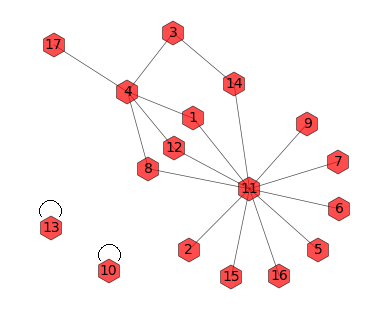
\includegraphics[width=400pt]{img/domesticaGraph.png}
    \caption{Grafo de Red Doméstica}
    \label{domesticaGraph}
\end{figure}

\textcolor{red}{COMPLETAR}

\subsubsection{Frecuencia de los distintos tipos de paquetes}

En el gr\'afico \ref{domesticaPaquetes} se pueden ver los resultados de obtenidos.

\begin{figure}[h!]
    \centering                                                       
    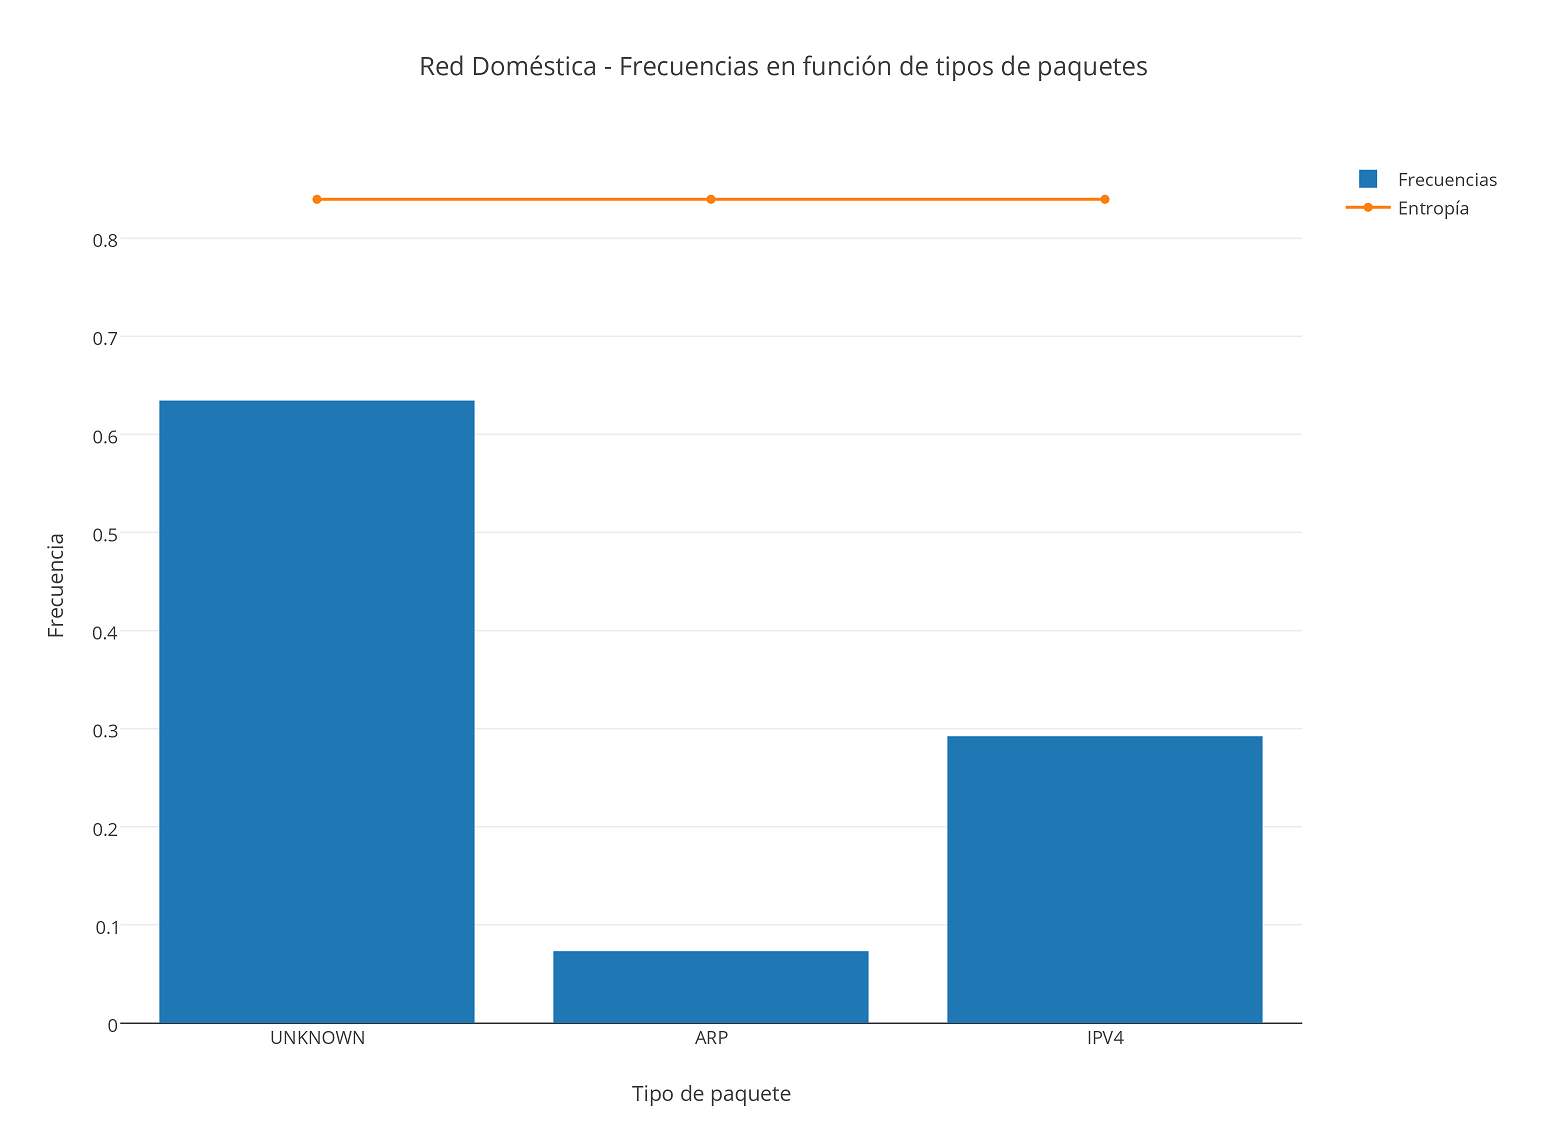
\includegraphics[width=400pt]{img/DomesticaFrecuenciaVsTipoPaquetes}
    \caption{}
    \label{domesticaPaquetes}
\end{figure}

\subsubsection{Informaci\'on de las fuentes emisoras y receptoras de paquetes ARP.}

Para realizar este caso comparamos la informaci\'on proporcionada por las fuentes emisoras de paquetes ARP e ilustramos asimismo la entrop\'ia de la fuente. Los resultados se pueden observar en los gr\'aficos \ref{domesticaEmisoras} y \ref{domesticaReceptoras}

\begin{figure}[h!]
    \centering                                                       
    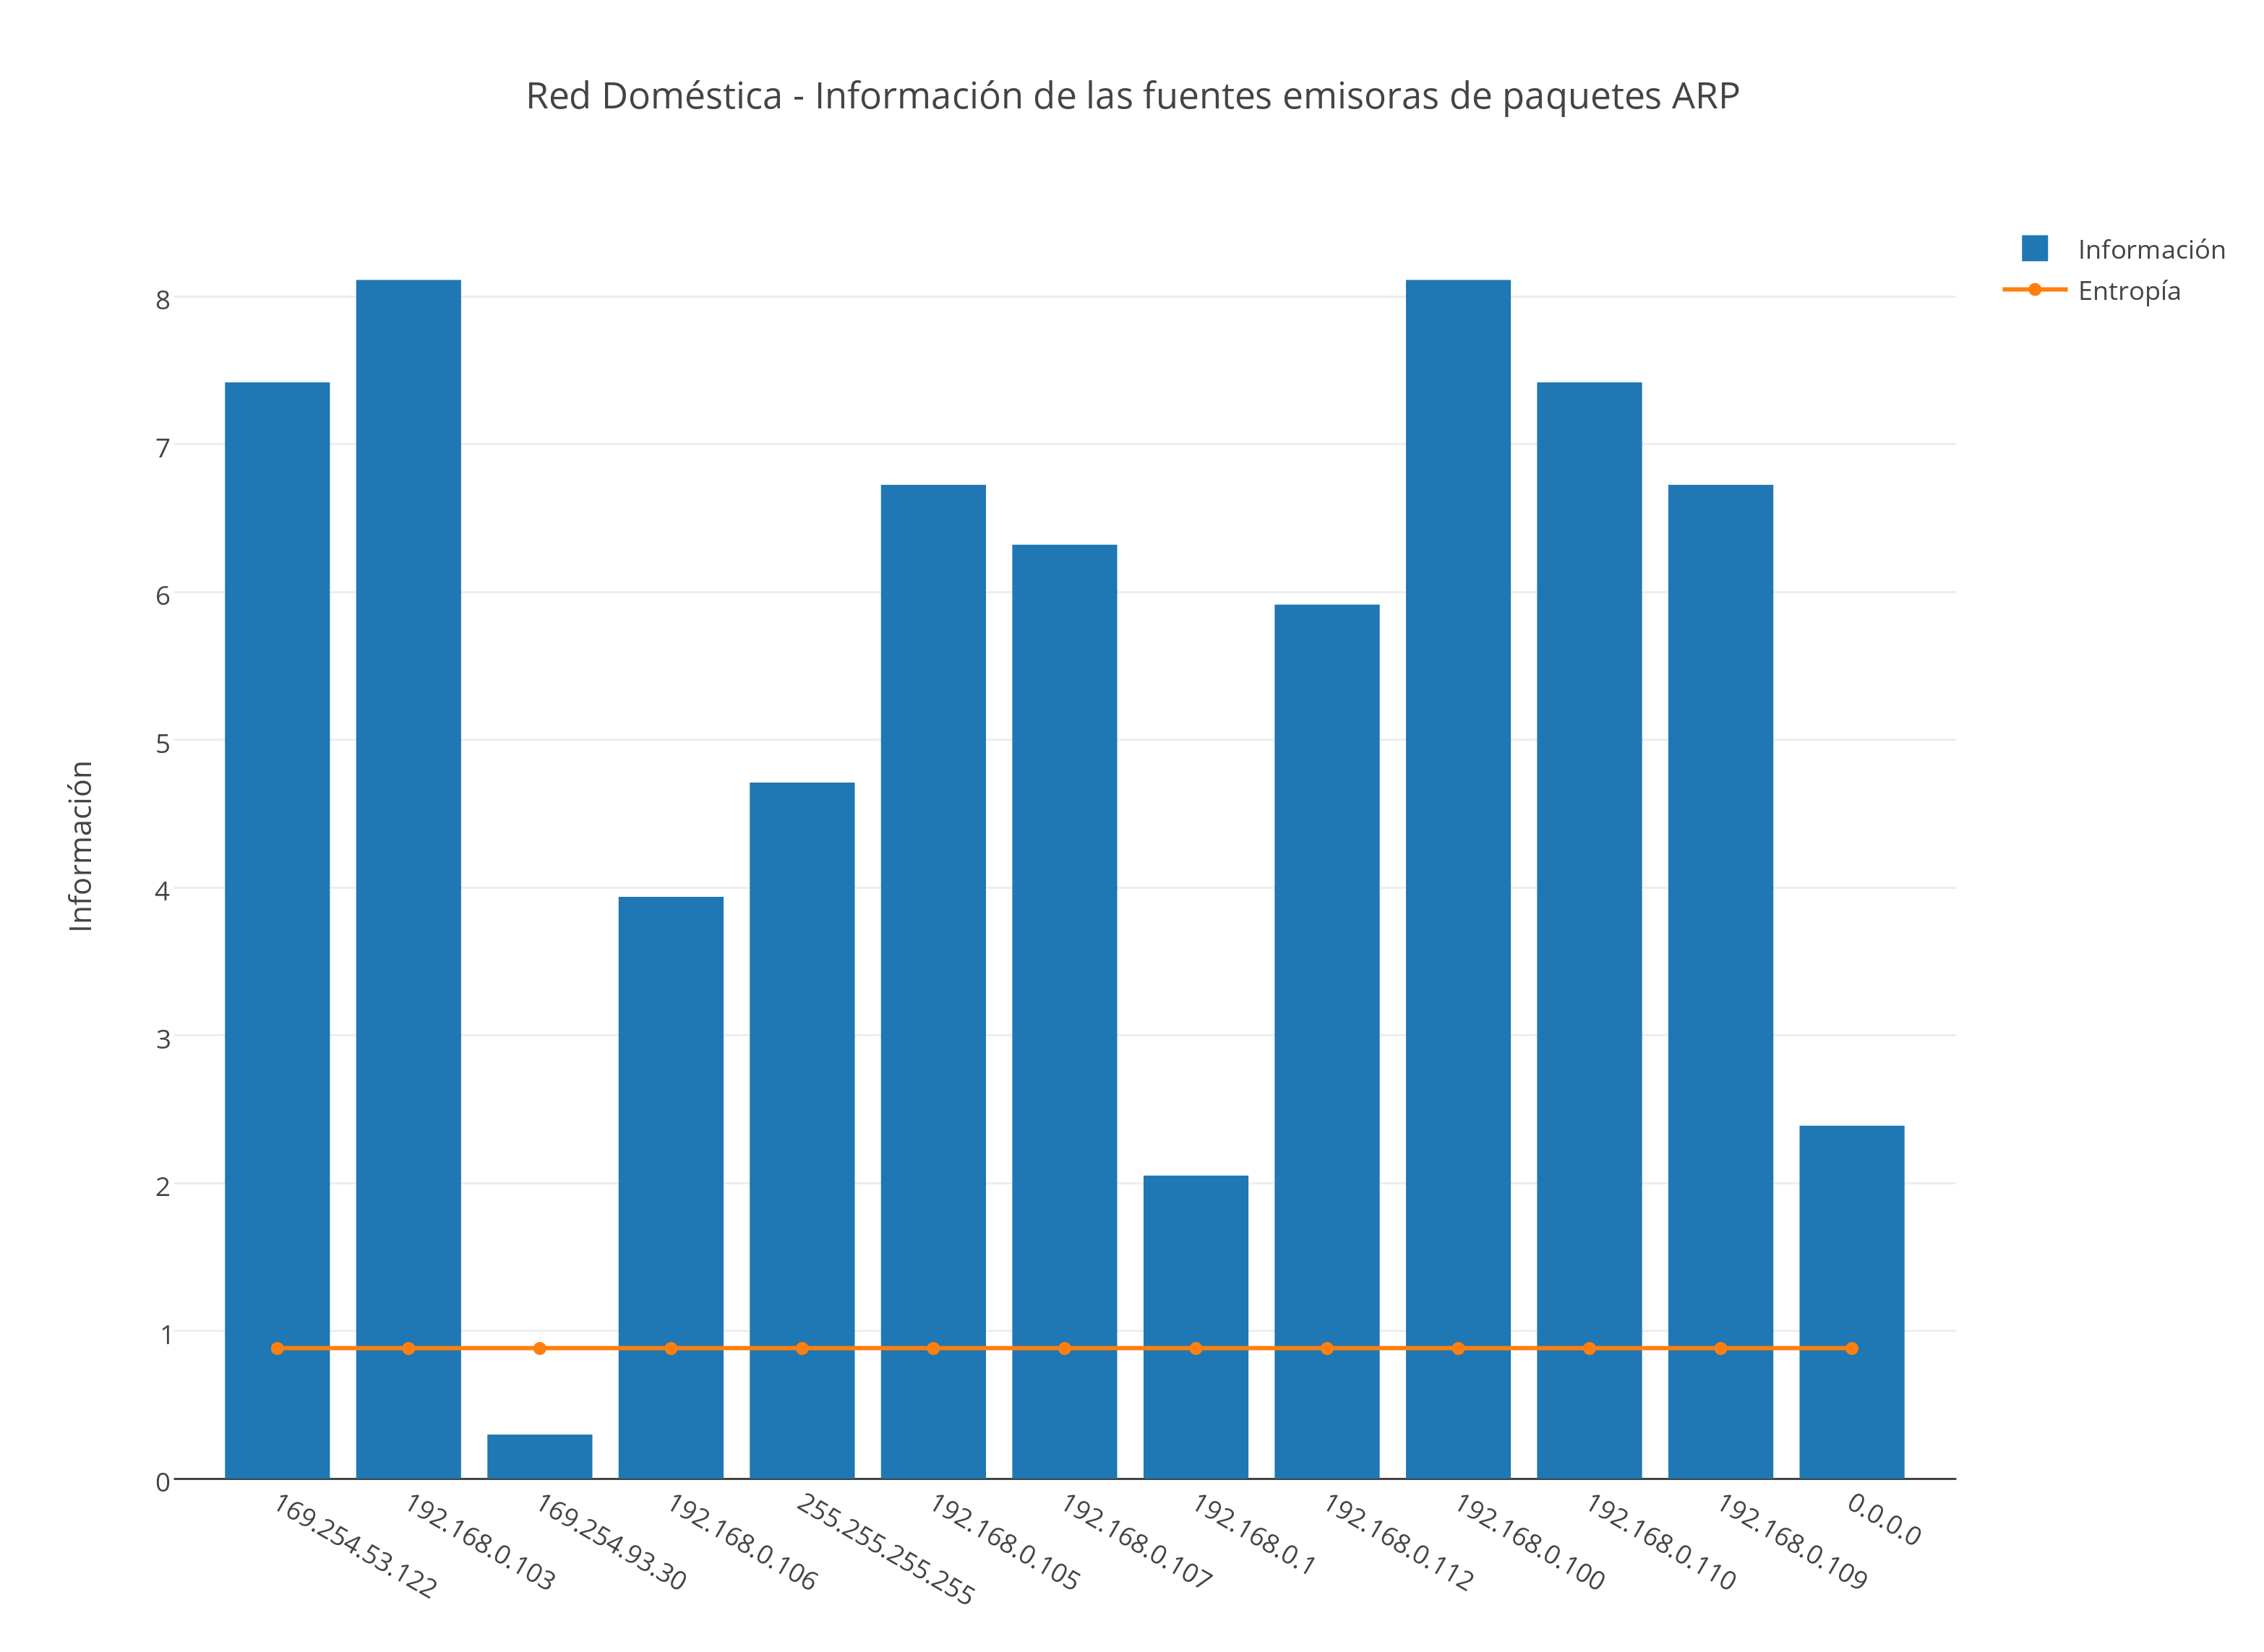
\includegraphics[width=400pt]{img/RedDomesticaFuentesEmisorasARP}
    \caption{}
    \label{domesticaEmisoras}
\end{figure}

En el primero de ellos se ve que existe una \'unica fuente situada por debajo de la entrop\'ia y corresponde a la IP 169.254.93.30. La baja informaci\'on que aporta indica que se trata de un nodo que emite muchos paquetes ARP. En contraposici\'on, las IP 192.168.0.103 y 192.168.0.100 muestran un gran aporte de informaci\'on, de lo cual se deduce que es poco com\'un que las mismas env\'ien paquetes de solicitud ARP.


\begin{figure}[h!]
    \centering                                                       
    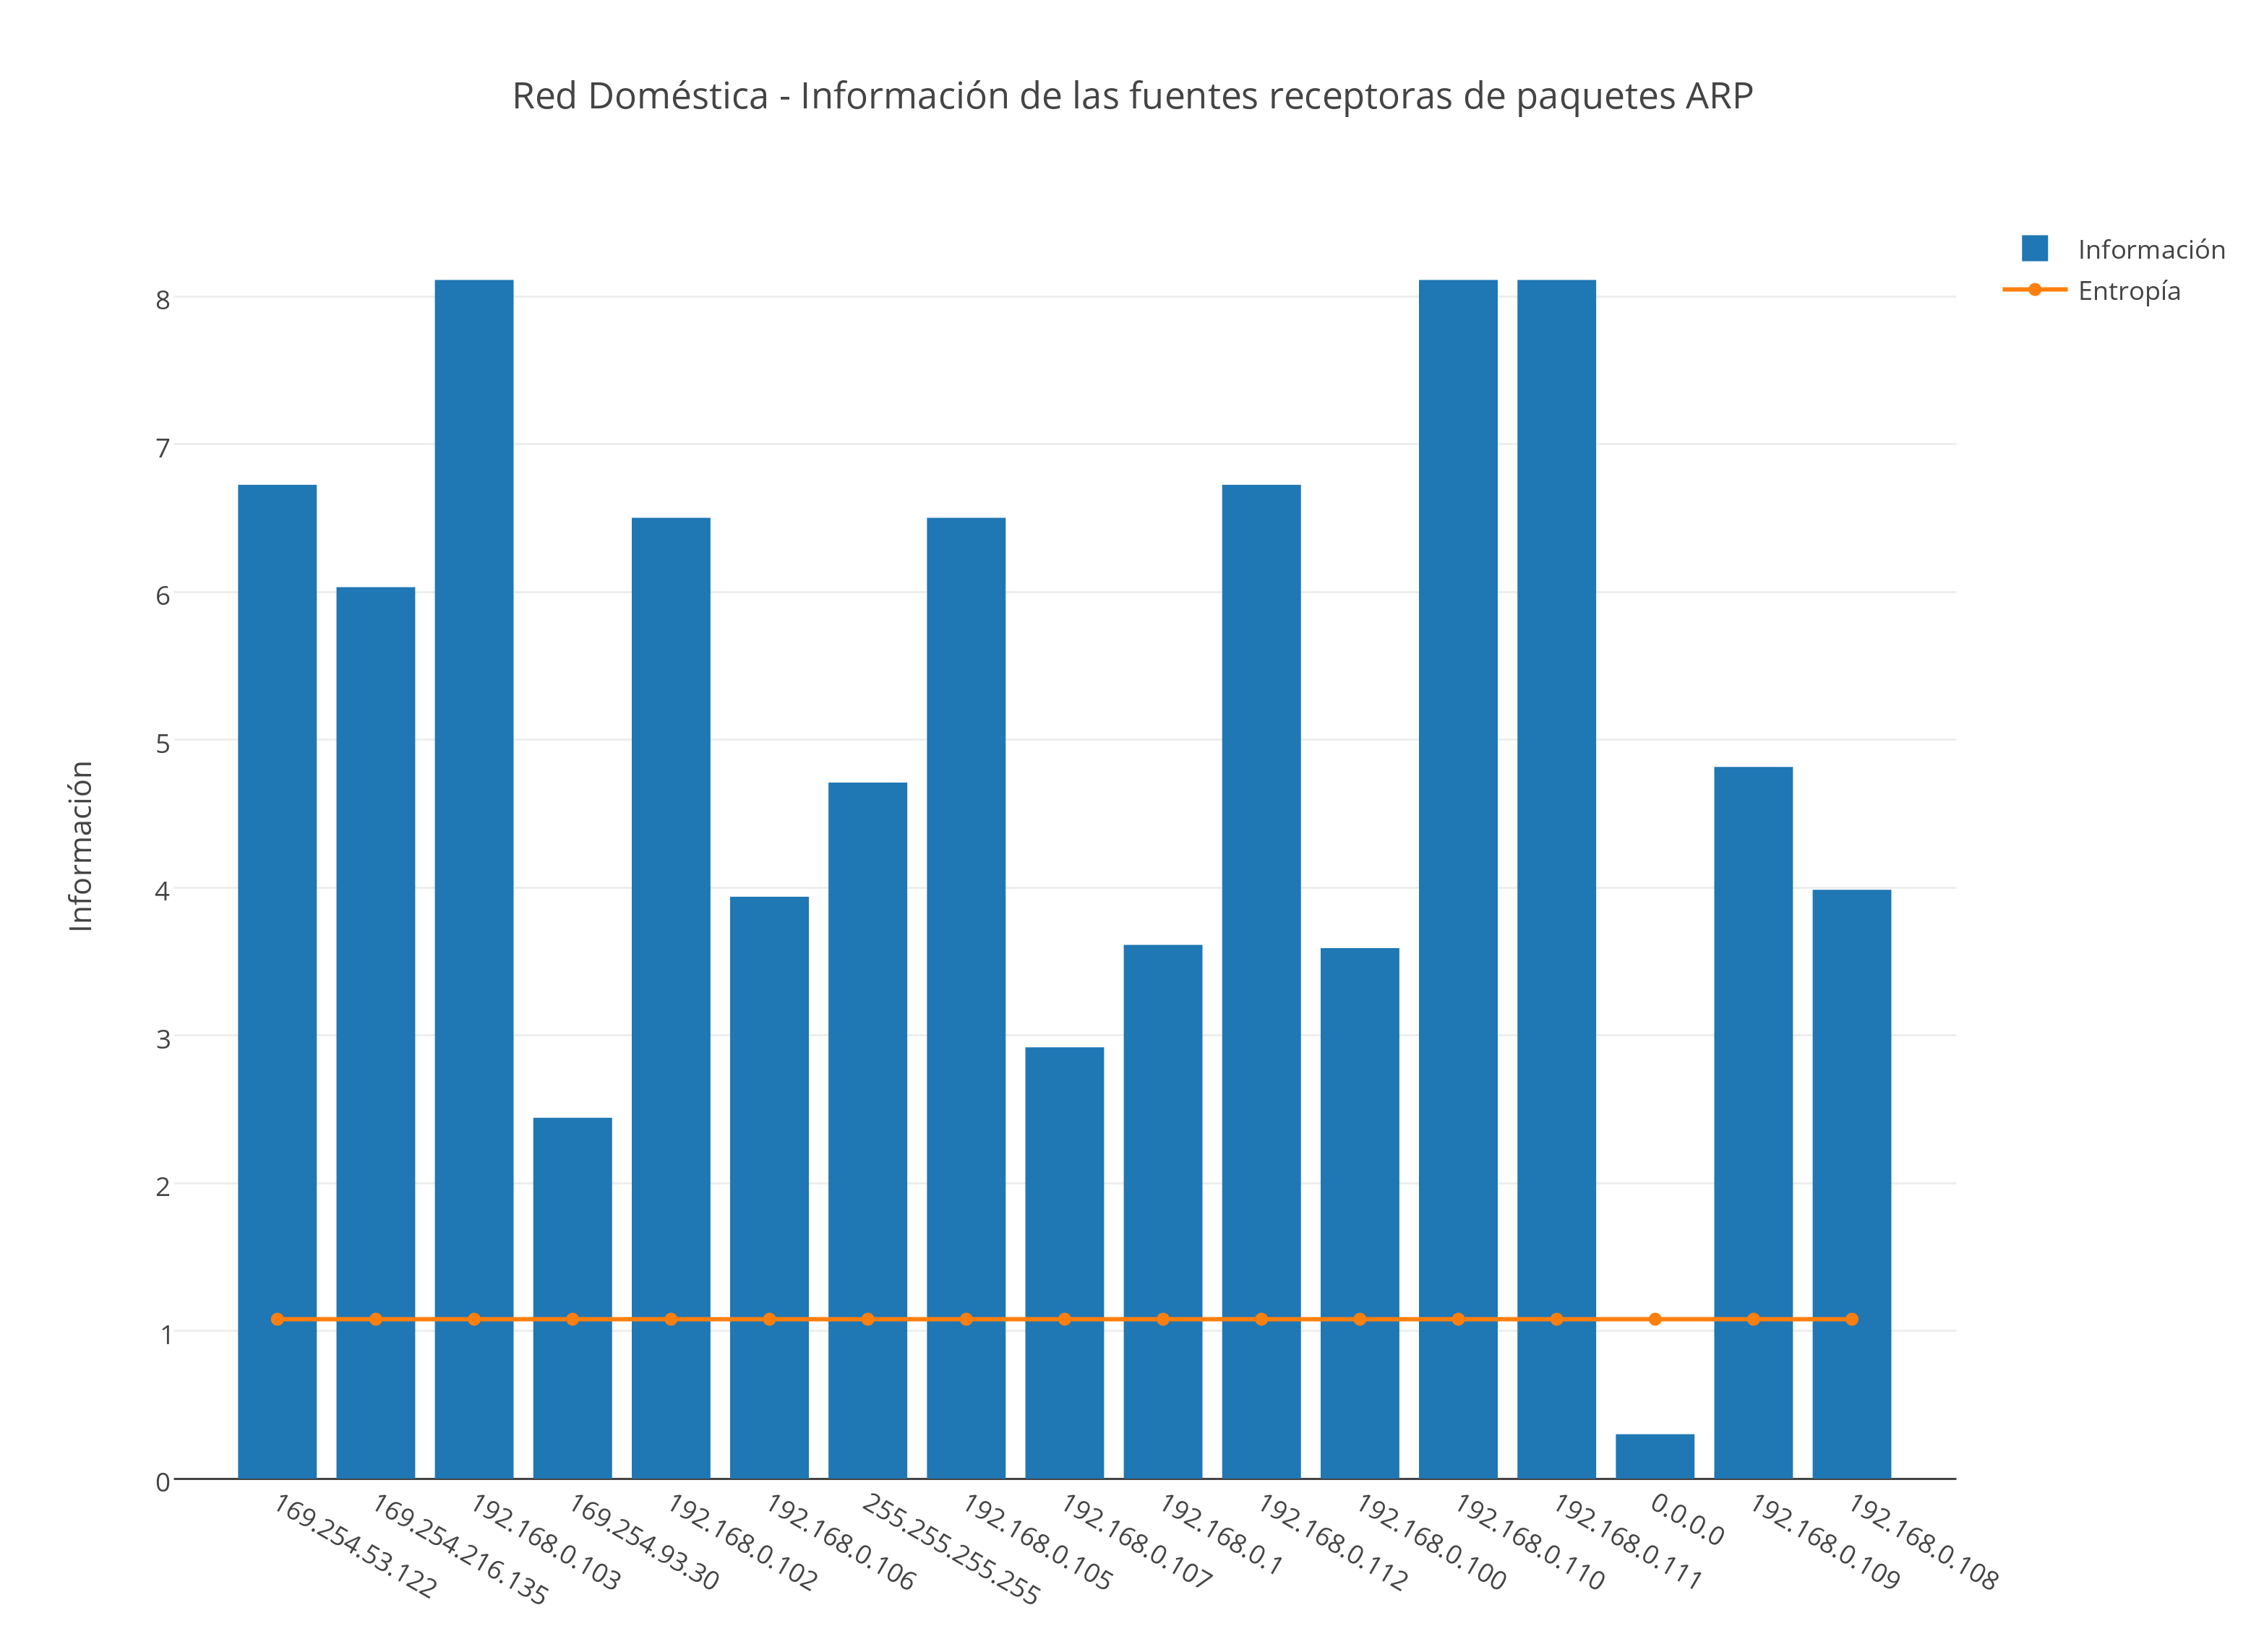
\includegraphics[width=400pt]{img/RedDomesticaFuentesReceptorasARP}
    \caption{}
    \label{domesticaReceptoras}
\end{figure}

En el segundo gr\'afico se observa una entrop\'ia mayor. De esto podr\'ia deducirse que es una fuente a\'un m\'as aleatoria y menos predecible que la que filtra \'unicamente los env\'ios de paquetes ARP.\\
En este caso, los nodos distinguidos son - por su gran valor de informaci\'on - los que mapean las direcciones IP 192.168.0.103, 192.168.0.9 y 192.168.0.111 y, por su poca cantidad de informaci\'on el nodo 0.0.0.0, seguido del 169.254.93.30. Esto indica que frecuentemente se realizan requests a estos \'ultimos hosts, mientras que los primeros son ignorados la mayor parte del tiempo. \\
\textcolor{red}{ver si tiene alguna relacion con la forma en q estan dispuestos en el grafo!}

¿Por qu\'e es tan frecuente que se realicen solicitudes al host cuya IP es 0.0.0.0? Podr\'iamos pensar que se trata de comunicaciones que un nodo env\'ia a s\'i mismo pero tambi\'en cabr\'ia suponer - de acuerdo a lo investigado - que puede tratarse de un mecanismo de chequeo de IP's duplicadas en la red.\\

Comparando ambos gr\'aficos podr\'iamos decir que es bastante com\'un que la IP 169.254.93.30 env\'ie y reciba paquetes ARP. Es por eso que consideramos que podr\'ia ser un potencial candidato a Router. \textcolor{red}{verificar con el grafo.}

\newpage
\subsection{Red Laboral}

En este segundo caso, se analiz\'o una red laboral de una PyME. La captura se realiz\'o por un lapso de media hora en modo promiscuo.

\subsubsection{Nodos intervinientes}
En el gr\'afico \ref{laboralGraph} se pueden ver los resultados de obtenidos.

\begin{figure}[h!]
    \centering                                                       
    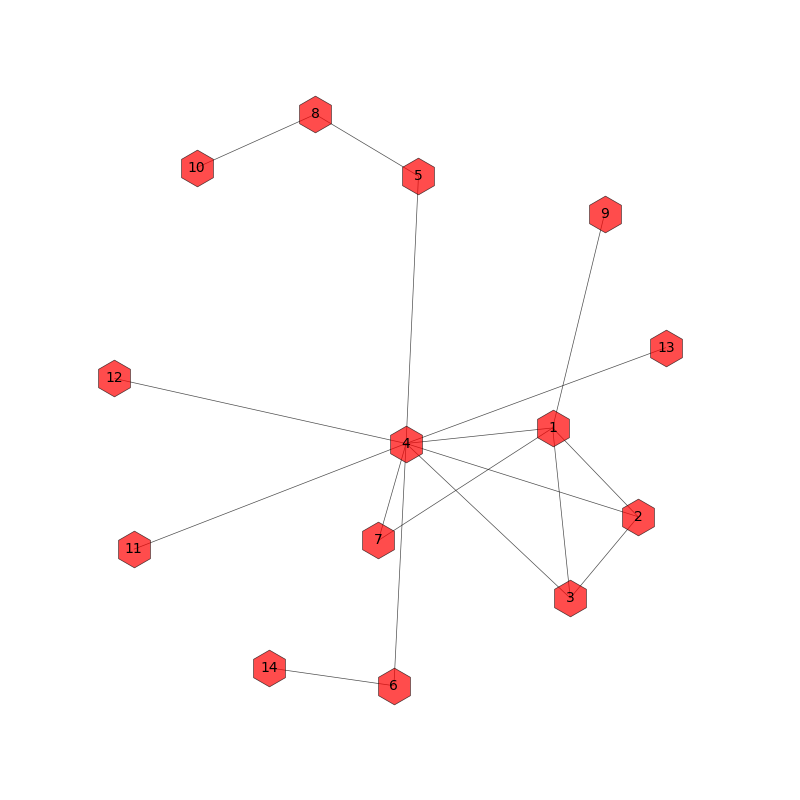
\includegraphics[width=400pt]{img/laboralGraph.png}
    \caption{Grafo de Red Laboral}
    \label{laboralGraph}
\end{figure}

La visualizaci\'on del grafo indicar\'ia, a primera vista, que el nodo 4 se transmite paquetes con la mayor\'ia de los dem\'as v\'ertices (excepto casos particulares) siendo el candidato ideal para ser el router de esta conexi\'on - es decir, el nodo con salida exterior.\\

El nodo 1 tambi\'en se comunica con varios nodos a la vez - esto se debe a que es un servidor local en la oficina, al cual le llegan peticiones de nodos particulares - que a su vez tambi\'en se comunican con los otros que acceden a dicho servidor local. Es decir, el nodo 2, 3, 7 y 9 acceden al servidor local 4, pero a su vez entre el 2 y el 3 se comunican entre ellos.\\

Los nodos 10, 8 y 14 parecieran ser nodos particulares que no se conectan con el router. En particular, el nodo 8 es 0.0.0.0, por lo que en realidad es el nodo 5 y 10 comunic\'andose con ellos mismos . El nodo 14 es una IP interna as\'i que posiblemente es un nodo comunic\'andose con una interfaz propia.\\

Luego de ese an\'alisis, consultamos las IPs con la configuraci\'on de la red (a la que tenemos acceso por ser la red de la oficina laboral). Efectivamente, el nodo 4 es el router, as\'i como el nodo 1 el servidor local estimado, y los nodos 2, 3, 7 y 9 los que se comunican con dicho servidor.

La incertidumbre del nodo 14 se resolvi\'o como una Virtual Network Adapter, producto de una Virtual Box corriendo en el nodo 6.

Todas las dem\'as relaciones parecen ser naturales, de nodos que se comunican con el router para poder salir a internet.

\subsubsection{Frecuencia de los distintos tipos de paquetes}

En el gr\'afico \ref{laboralPaquetes} se pueden ver los resultados de obtenidos. All\'i se observa la predominancia de los paquetes de tipo IPV4. Esto tiene sentido, puesto que en este contexto es m\'as frecuente el intercambio de paquetes a nivel de Internet que el realiazado a nivel de la intranet, con la cual las computadoras se encuentran conectadas a trav\'es de Ethernet \textcolor{red}{ESTO ES ASI? CORREGIR SI NO POR FAVOR}.

\begin{figure}[h!]
    \centering                                                       
    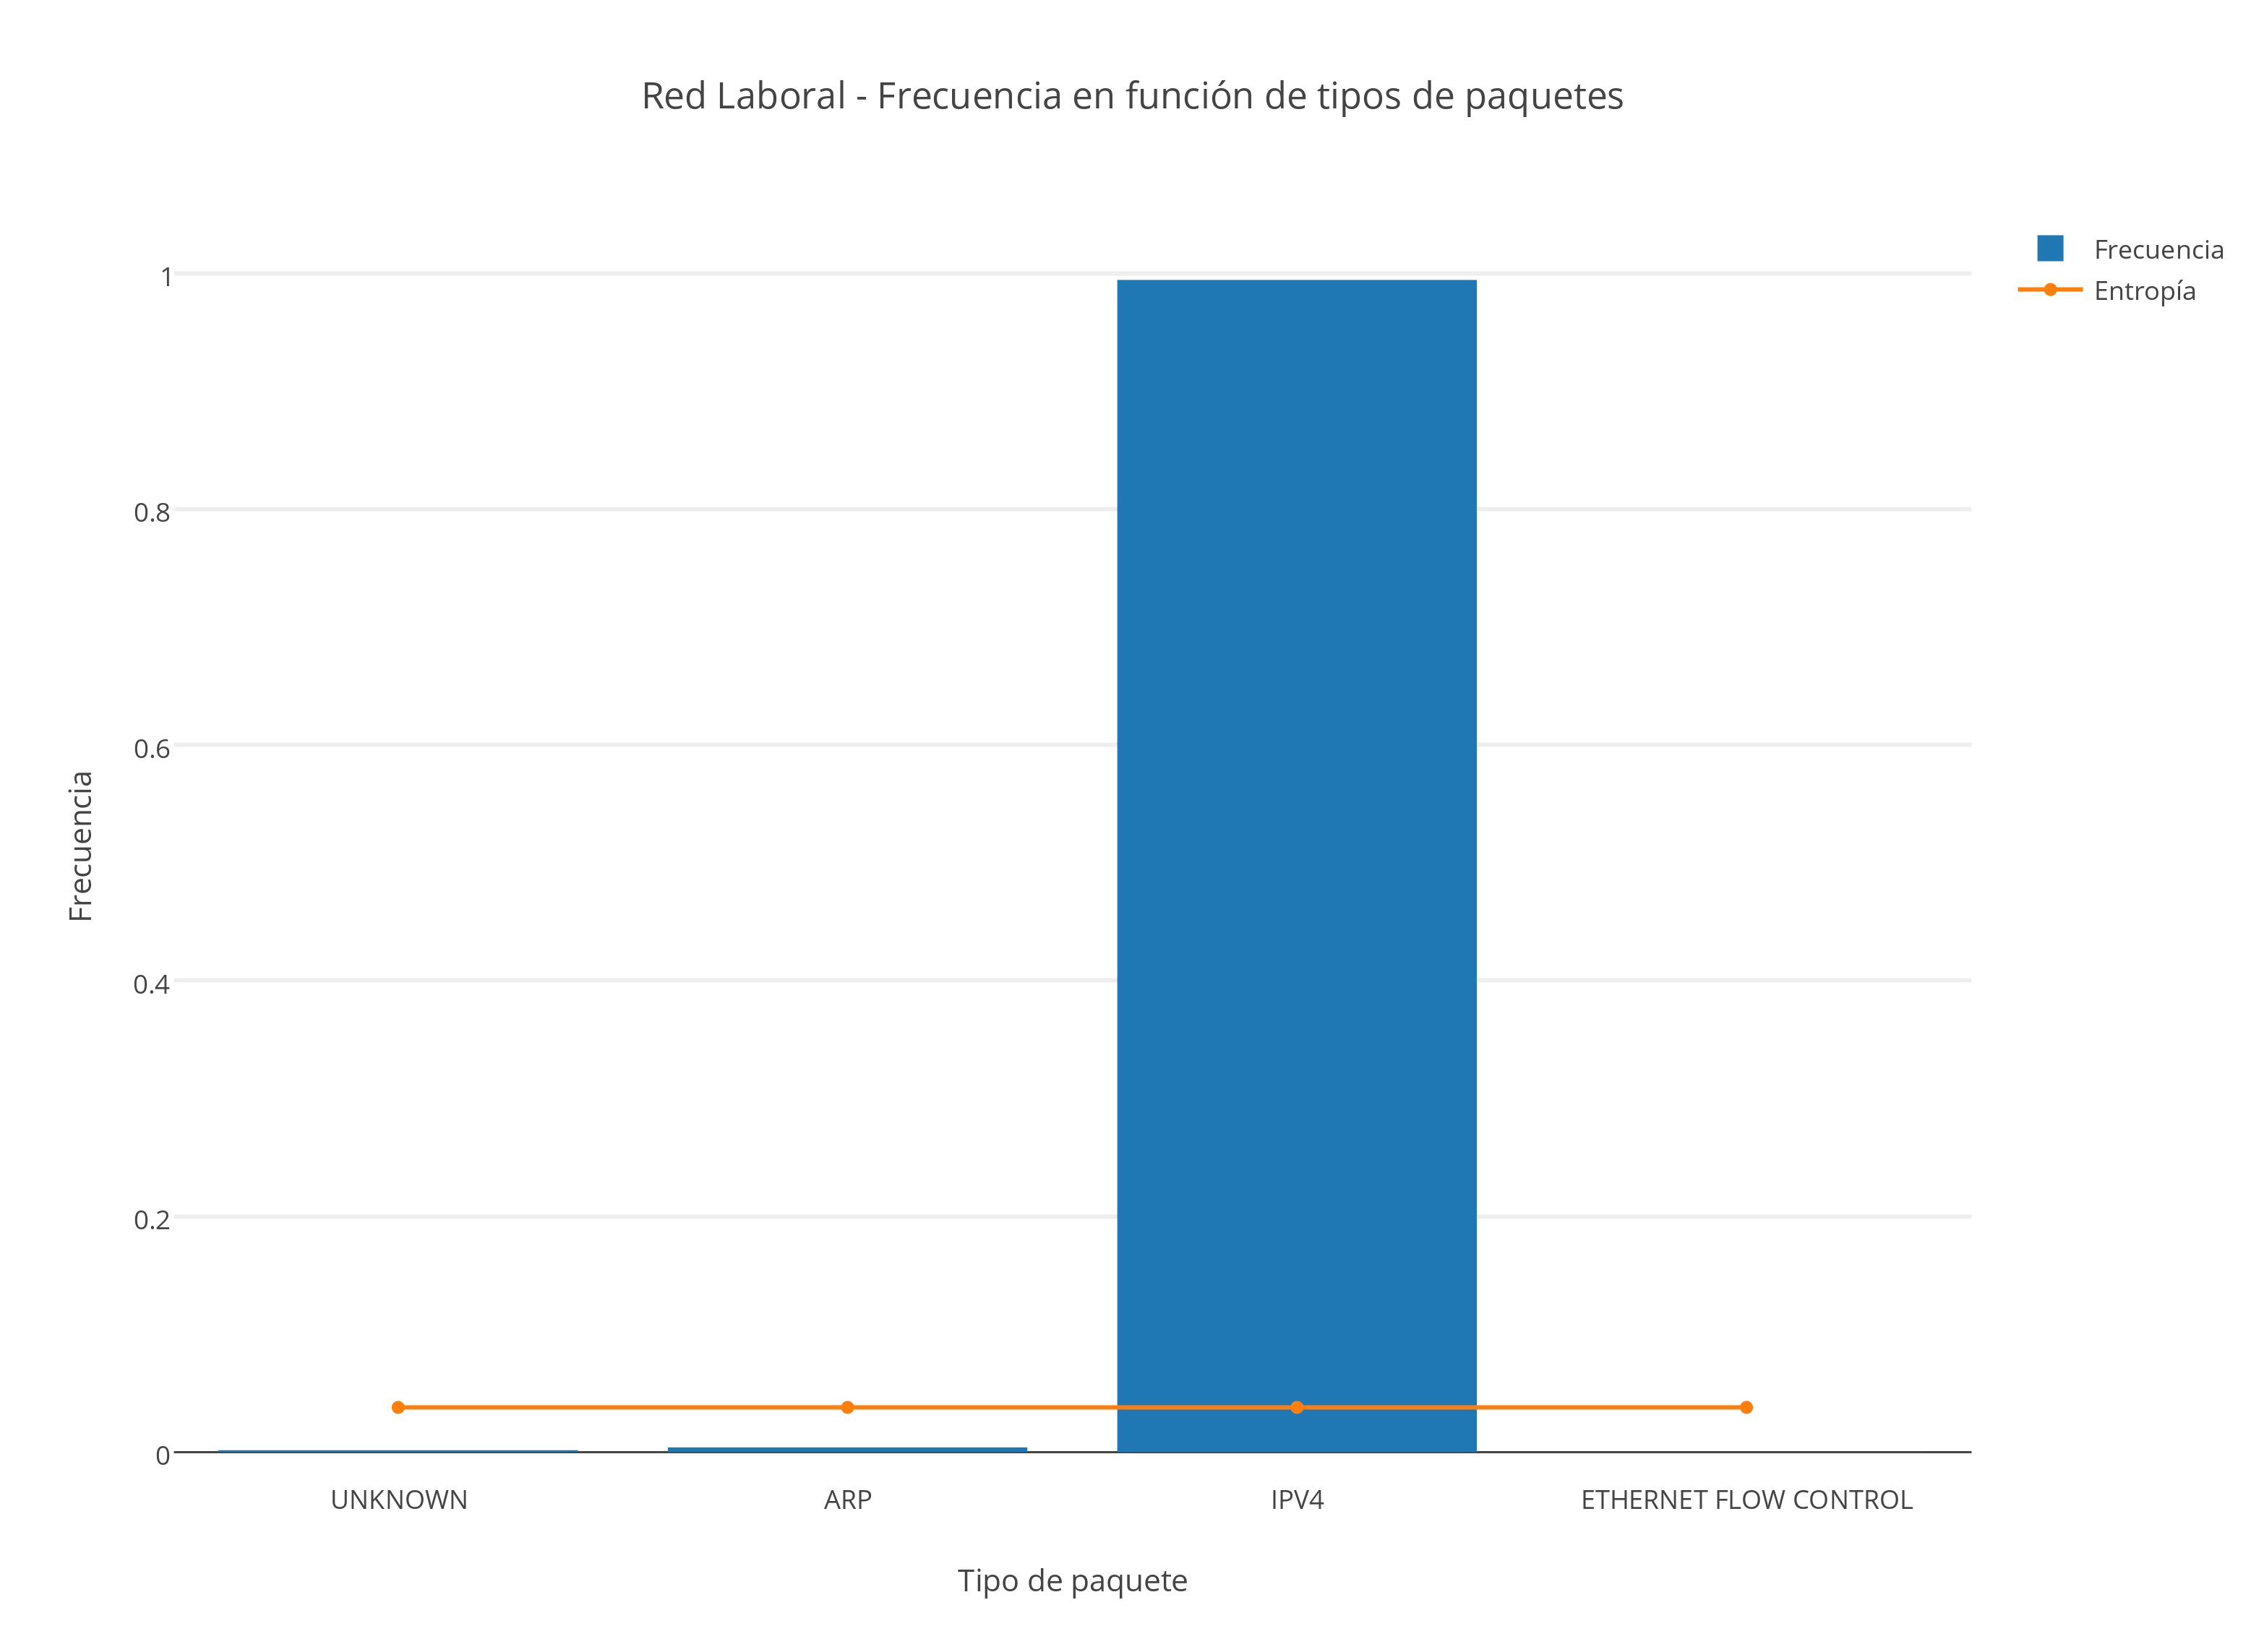
\includegraphics[width=400pt]{img/LaboralFrecuenciaVsTipoPaquetes}
    \caption{}
    \label{laboralPaquetes}
\end{figure}

Comparando las figuras \ref{laboralEmisoras} y \ref{laboralReceptoras} se puede ver que las fuentes receptoras superan en cantidad a las fuentes emisoras.\\

\subsubsection{Informaci\'on de las fuentes emisoras y receptoras de paquetes ARP.}

\begin{figure}[h!]
    \centering                                                       
    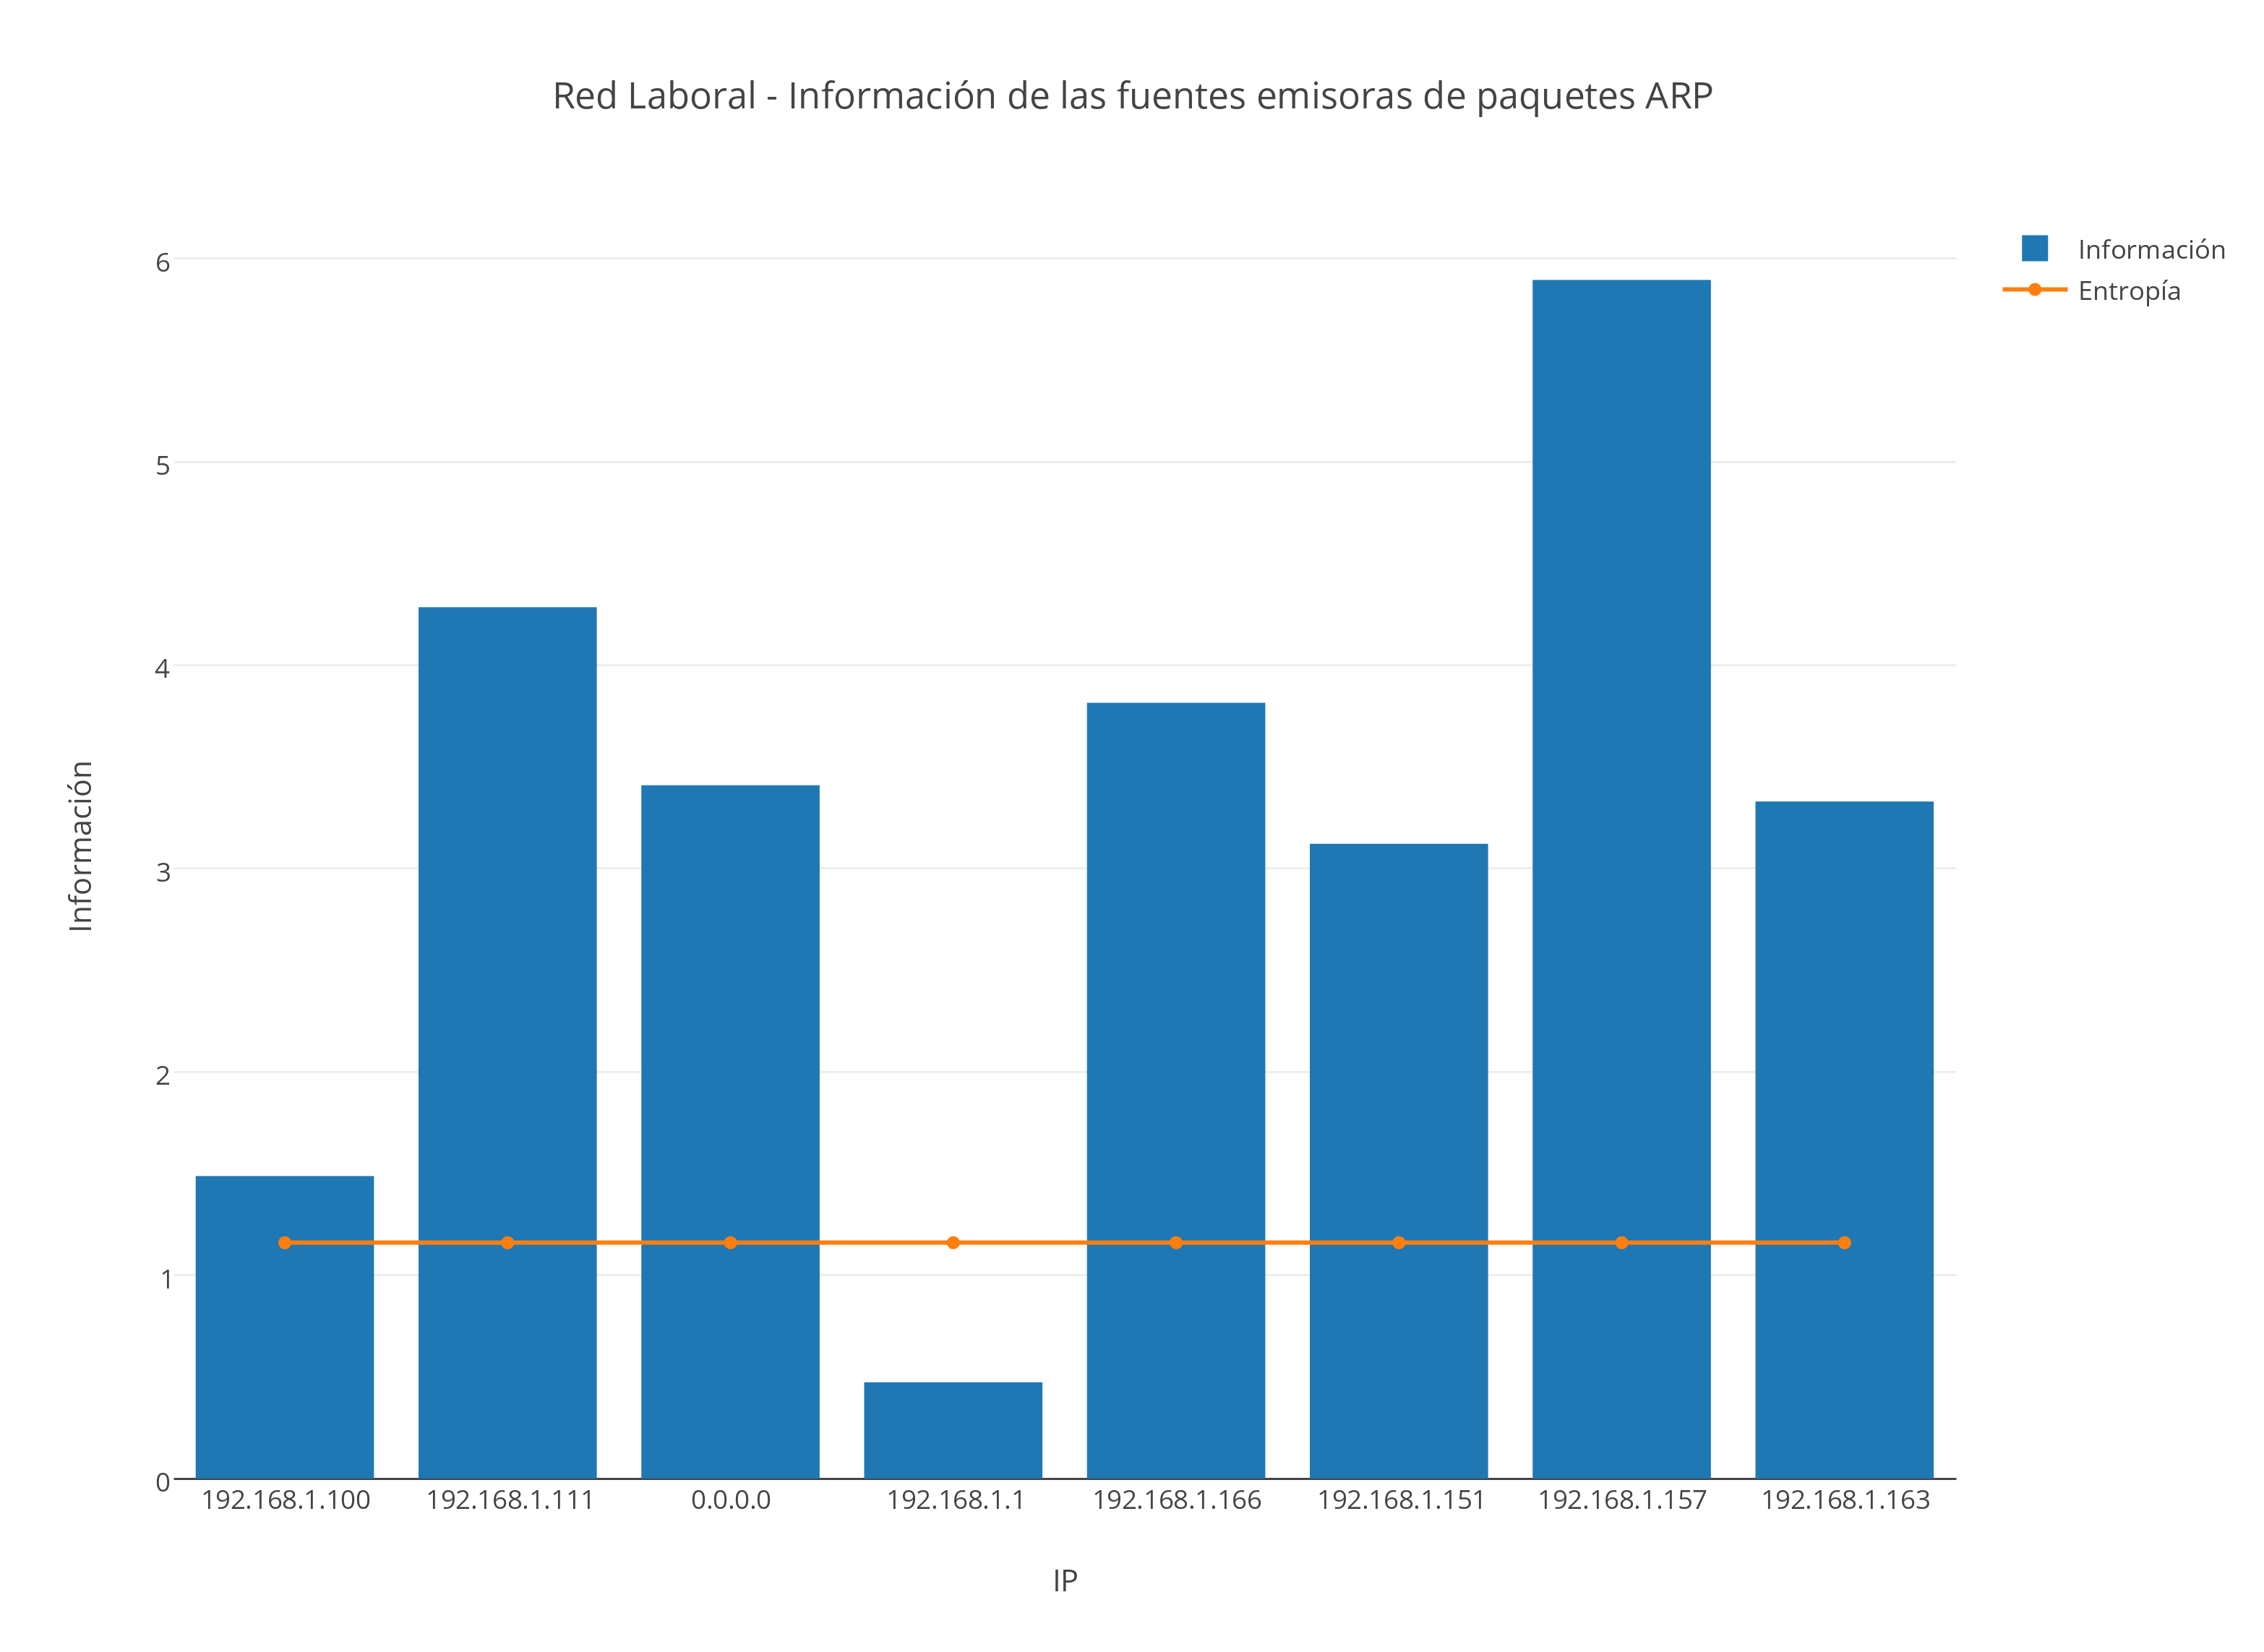
\includegraphics[width=400pt]{img/RedLaboralFuentesEmisorasARP}
    \caption{}
    \label{laboralEmisoras}
\end{figure}

Dentro de las IPs emisoras se puede destacar la participaci\'on activa de el nodo 192.168.1.1, la cu\'al aporta un valor muy pequeño de informaci\'on, encontr\'andose por debajo de la entrop\'ia. Esto indicar\'ia que se trata del host que m\'as paquetes ARP env\'ia dentro de la red. \\

\begin{figure}[h!]
    \centering                                                       
    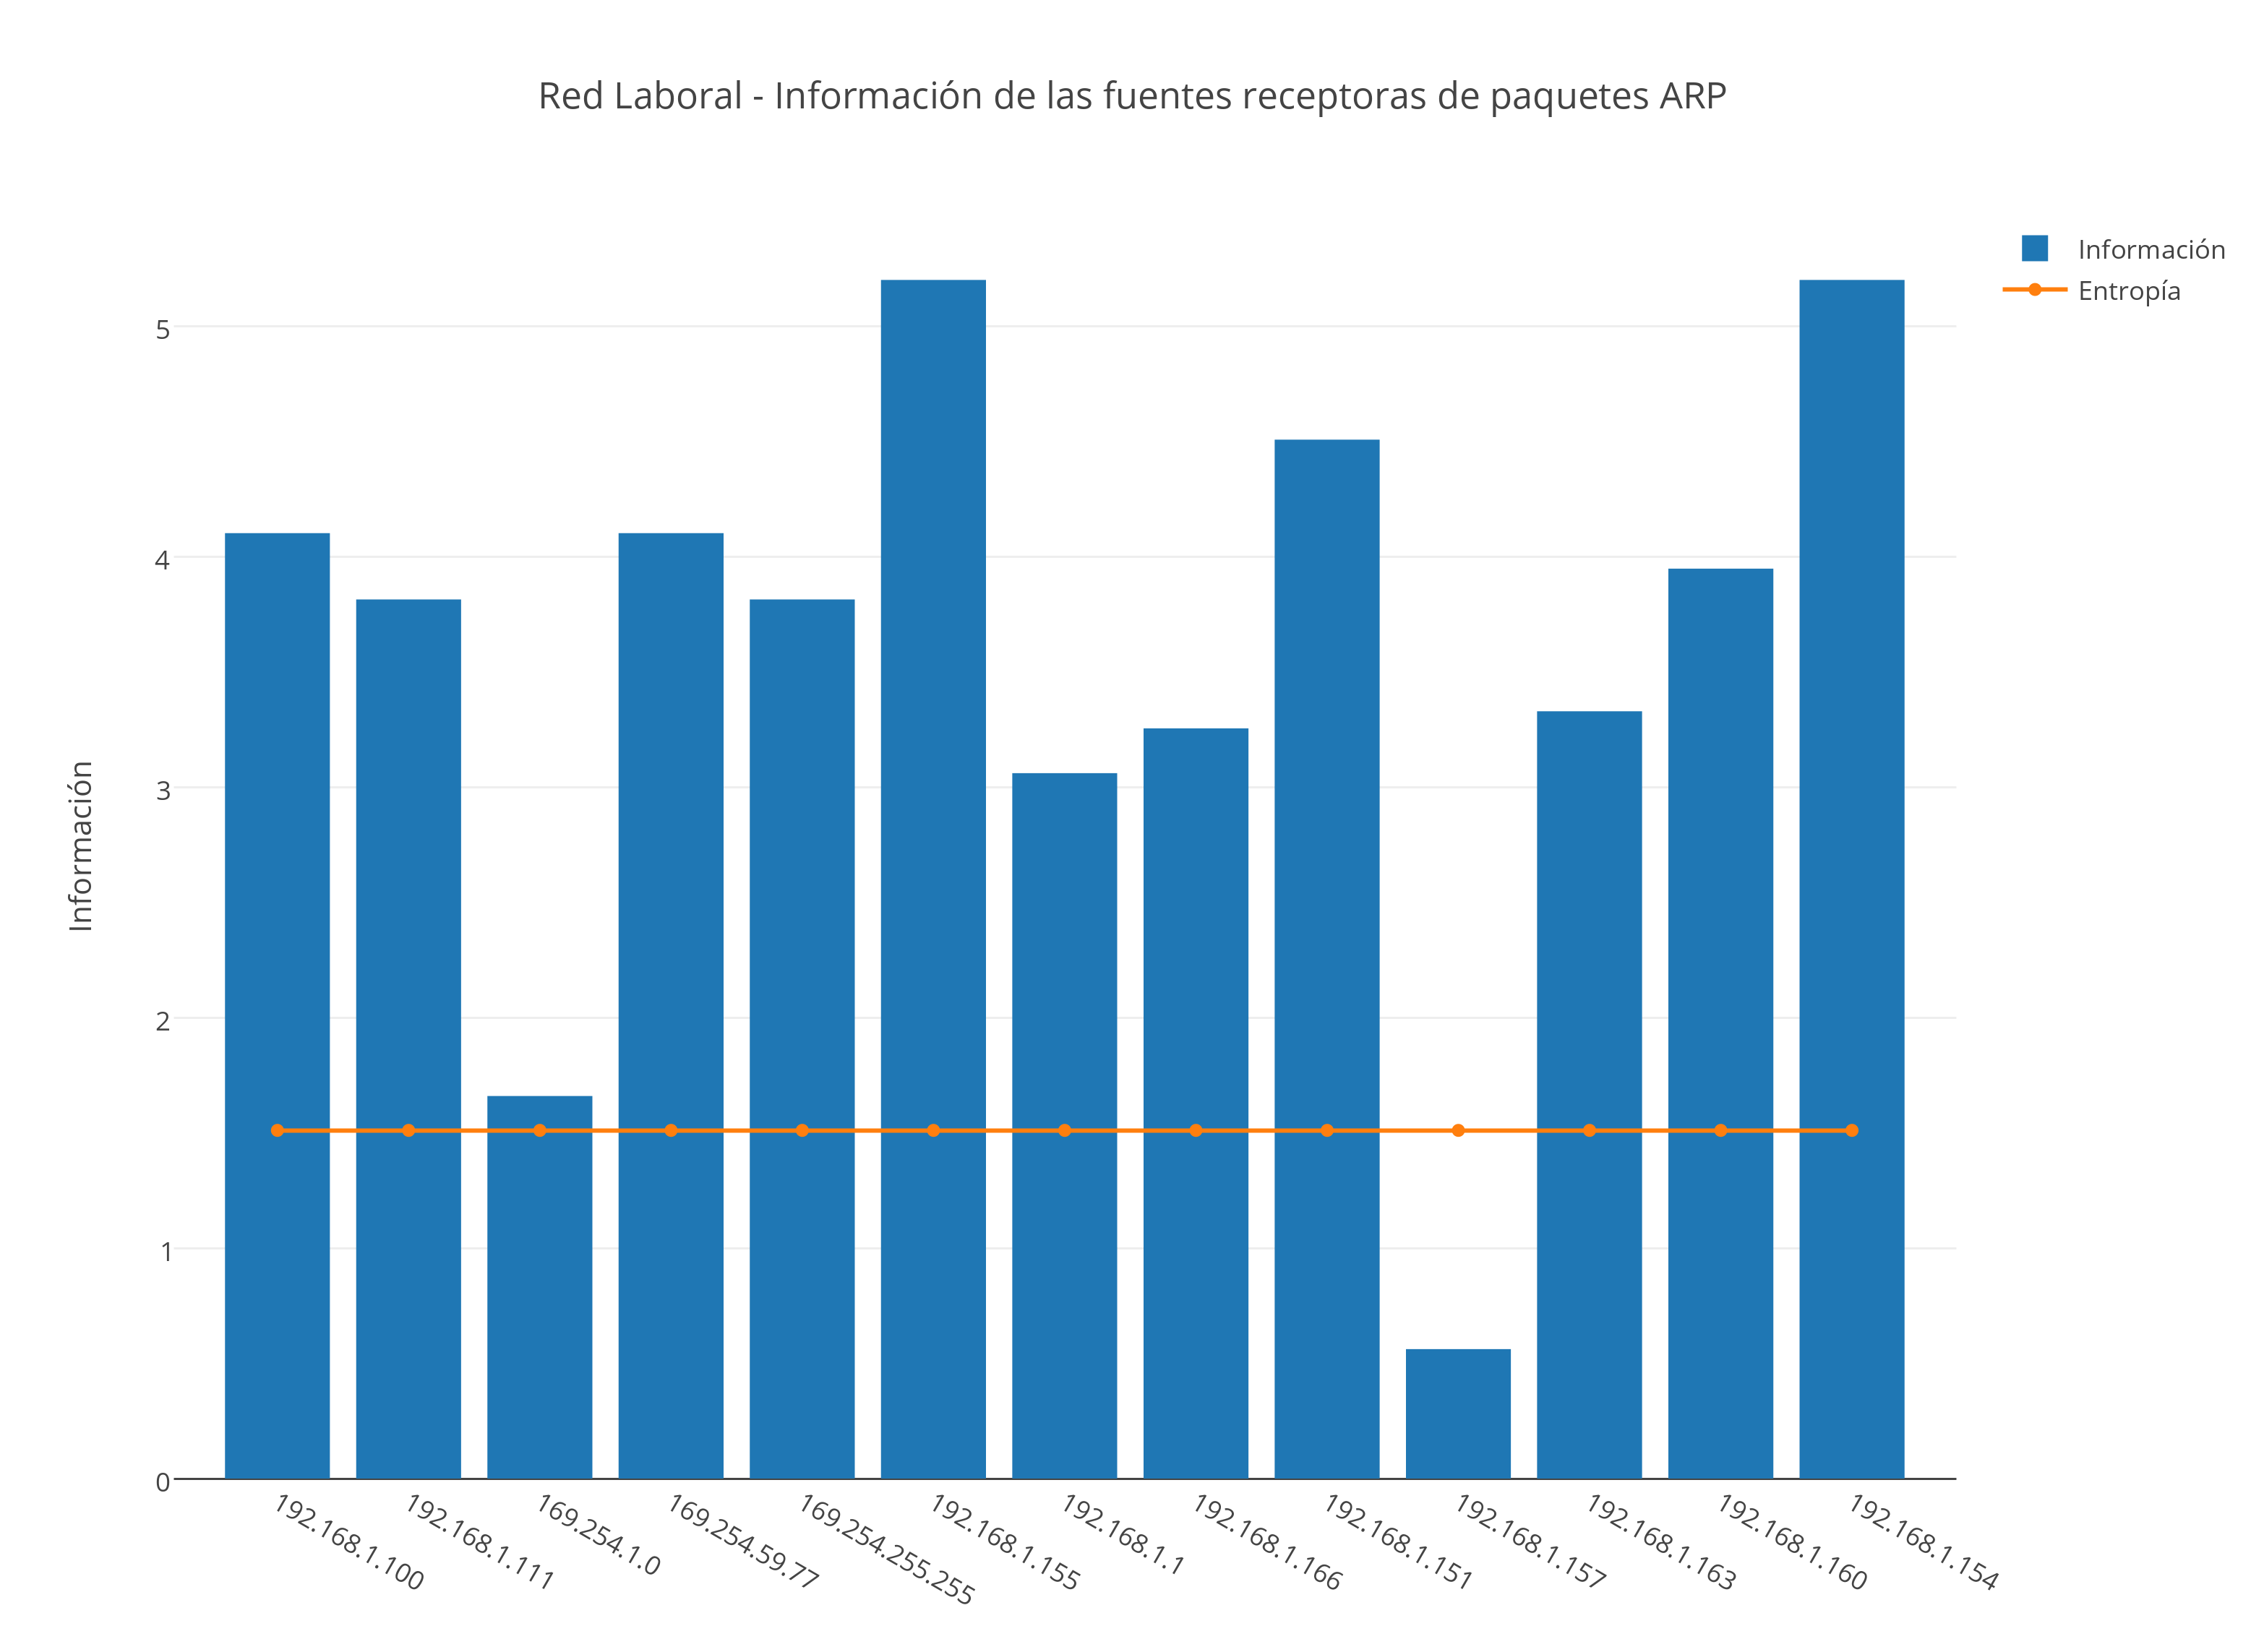
\includegraphics[width=400pt]{img/RedLaboralFuentesReceptorasARP}
    \caption{}
    \label{laboralReceptoras}
\end{figure}

Si lo buscamos en el gr\'afico \ref{laboralReceptoras}, el mismo nodo aporta una informaci\'on por encima de la media, pero sin ser destacada. Esto puede deberse a que se trata del Router, el cual debe encargarse de hacer llegar a todo v\'ertice de la red que coordina los mensajes que se transmiten a trav\'es de \'el.\\
Otro caso a destacar es el de la IP 192.168.1.157 (nodo 7). Este nodo se encuentra en la figura \ref{laboralReceptoras} como aquel que menos informaci\'on reporta, es decir, como el que m\'as frecuentemente recibe requests. \\ \textcolor{red}{POR QUE SERA ASI SI NO ES NI SERVER NI ROUTER? NO SE COMO EXPLICARLO}


\newpage
\subsection{Red Bonafide}
 Por \'ultimo, dadas las peque\~nas dimensiones de las redes anteriores, decidimos tomar datos de la red p\'ublica ofrecida por el local Bonafide. La captura se realiz\'o por un lapso de media hora en modo promiscuo.

\subsubsection{Nodos intervinientes}

En el gr\'afico \ref{bonafideGraph} se pueden ver los resultados de obtenidos.

\begin{figure}[h!]
    \centering                                                       
    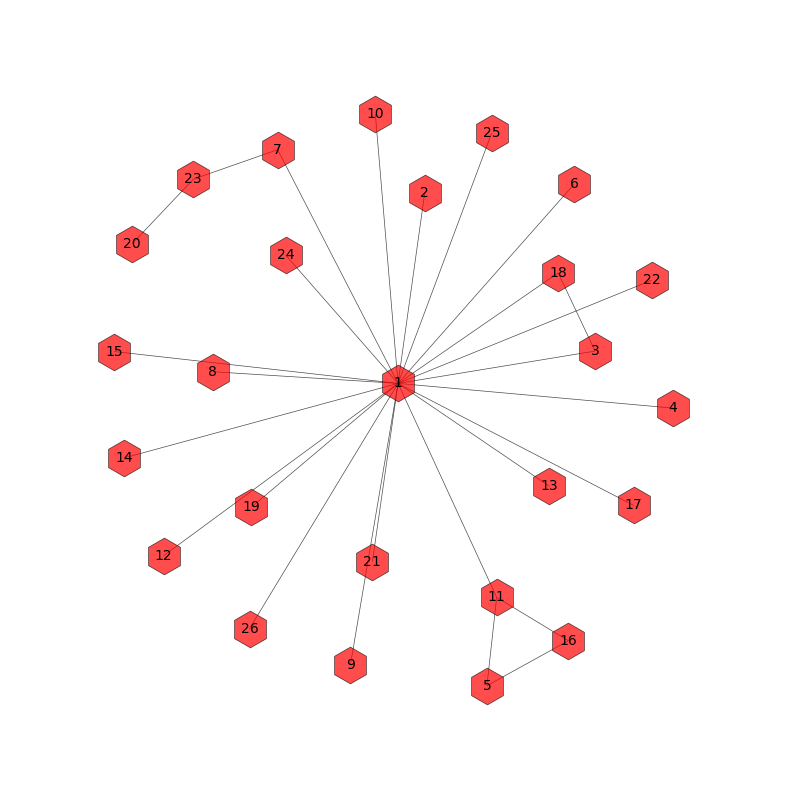
\includegraphics[width=400pt]{img/bonafideGraph.png}
    \caption{Grafo de Red Bonafide}
    \label{bonafideGraph}
\end{figure}
Si bien el grafo resultante no es exactamente la idea previa que ten\'iamos de \'el (un grafo estrella con el nodo root como ra\'iz) resulta interesante observar la indiscutible predominancia de aristas incidentes al nodo 1, descripto con la direcci\'on IP 192.168.1.1: el resto de los nodos son adyacentes a \'el o tienen un camino al mismo de - a lo sumo - tercer grado.\\
Consideramos que estos datos son suficientes como para deducir que dicha direcci\'on IP coincide con la del router.\\
Al indagar acerca de la naturaleza de los \'unicos nodos que no se encuentran conectados de forma directa al nodo 1 (el 5 (192.168.1.110), el 16 (192.168.1.4), el 23(0.0.0.0) y el 20 (169.254.201.232)) llegamos a las siguientes conclusiones: \\
\begin{itemize}
	\item Tanto el nodo 5 como el 16 (ambos de clase C) se comunican con el router a trav\'es del nodo 11 (192.168.1.105). Ahondando en las caracter\'isticas de estas transferencias, se puede ver que el nodo 11 realiza requests a los nodos 1, 5 y 16, pero s\'olo llega a \'el un request desde el nodo 16. Podr\'iamos entonces inferir que el nodo 11 puede estar funcionando como switch \textcolor{red}{FRUTA FRUTA FRUTA PARA TODOS. AVERIGUAR ESTO Y CORREGIRLO.}
	\item El nodo 20 se conecta al 23 y \'este \'ultimo al 7 (192.168.1.100). Esto forma la secuencia 169.254.201.232 (clase B)- 0.0.0.0 - 192.168.1.100 (clase C) - router. Si bien no se trata de un grafo dirigido, se puede ver en los resultados que la direcci\'on 0.0.0.0 nunca recibe datos que podamos escuchar, si no que env\'ia requests a ambos nodos que lo circundan.\\ De acuerdo a lo investigado, inferimos que se trata de un fen\'omeno que ocurre cuando un nuevo host se conecta a la IP, con el fin de verificar que no tenga una direcci\'on que se encuentre en uso, evitando as\'i las IP duplicadas.\\
\end{itemize}


\subsubsection{Frecuencia de los distintos tipos de paquetes}

En el gr\'afico \ref{bonafidePaquetes} se pueden ver los resultados de obtenidos.

\begin{figure}[h!]
    \centering                                                       
    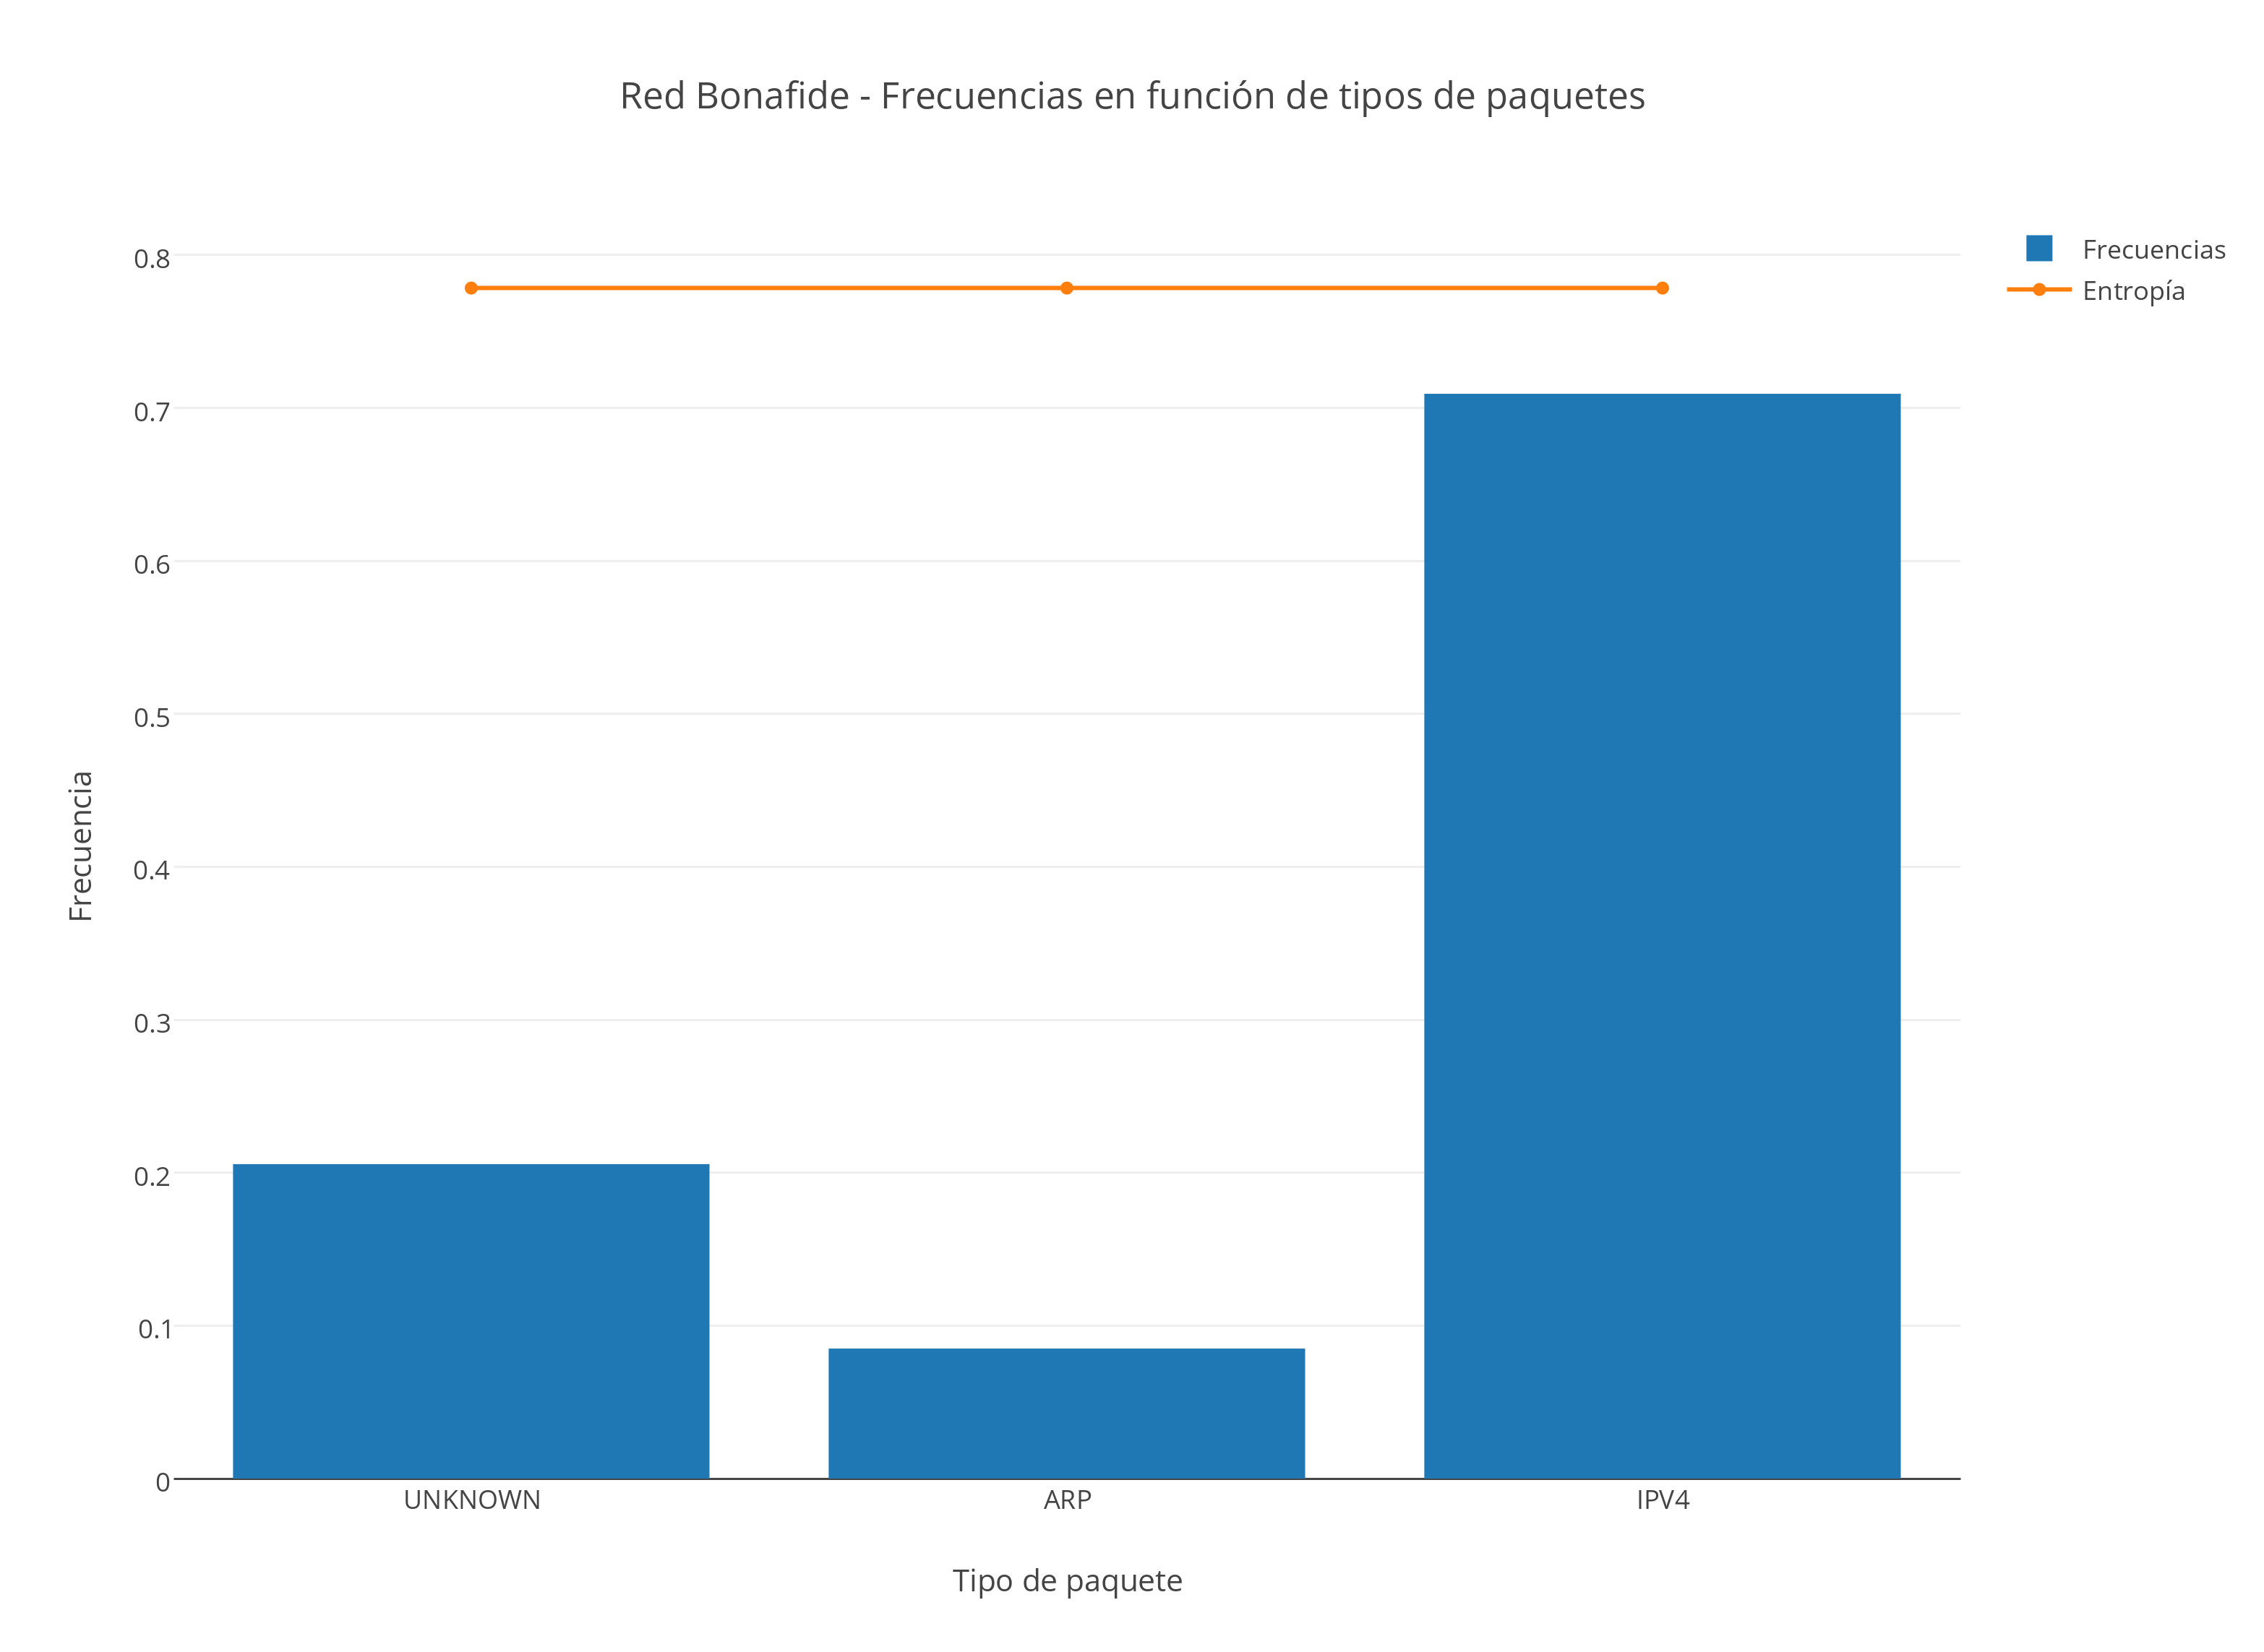
\includegraphics[width=400pt]{img/BonafideFrecuenciaVsTipoPaquetes}
    \caption{}
    \label{bonafidePaquetes}
\end{figure}

\subsubsection{Informaci\'on de las fuentes emisoras y receptoras de paquetes ARP.}

\begin{figure}[h!]
    \centering                                                       
    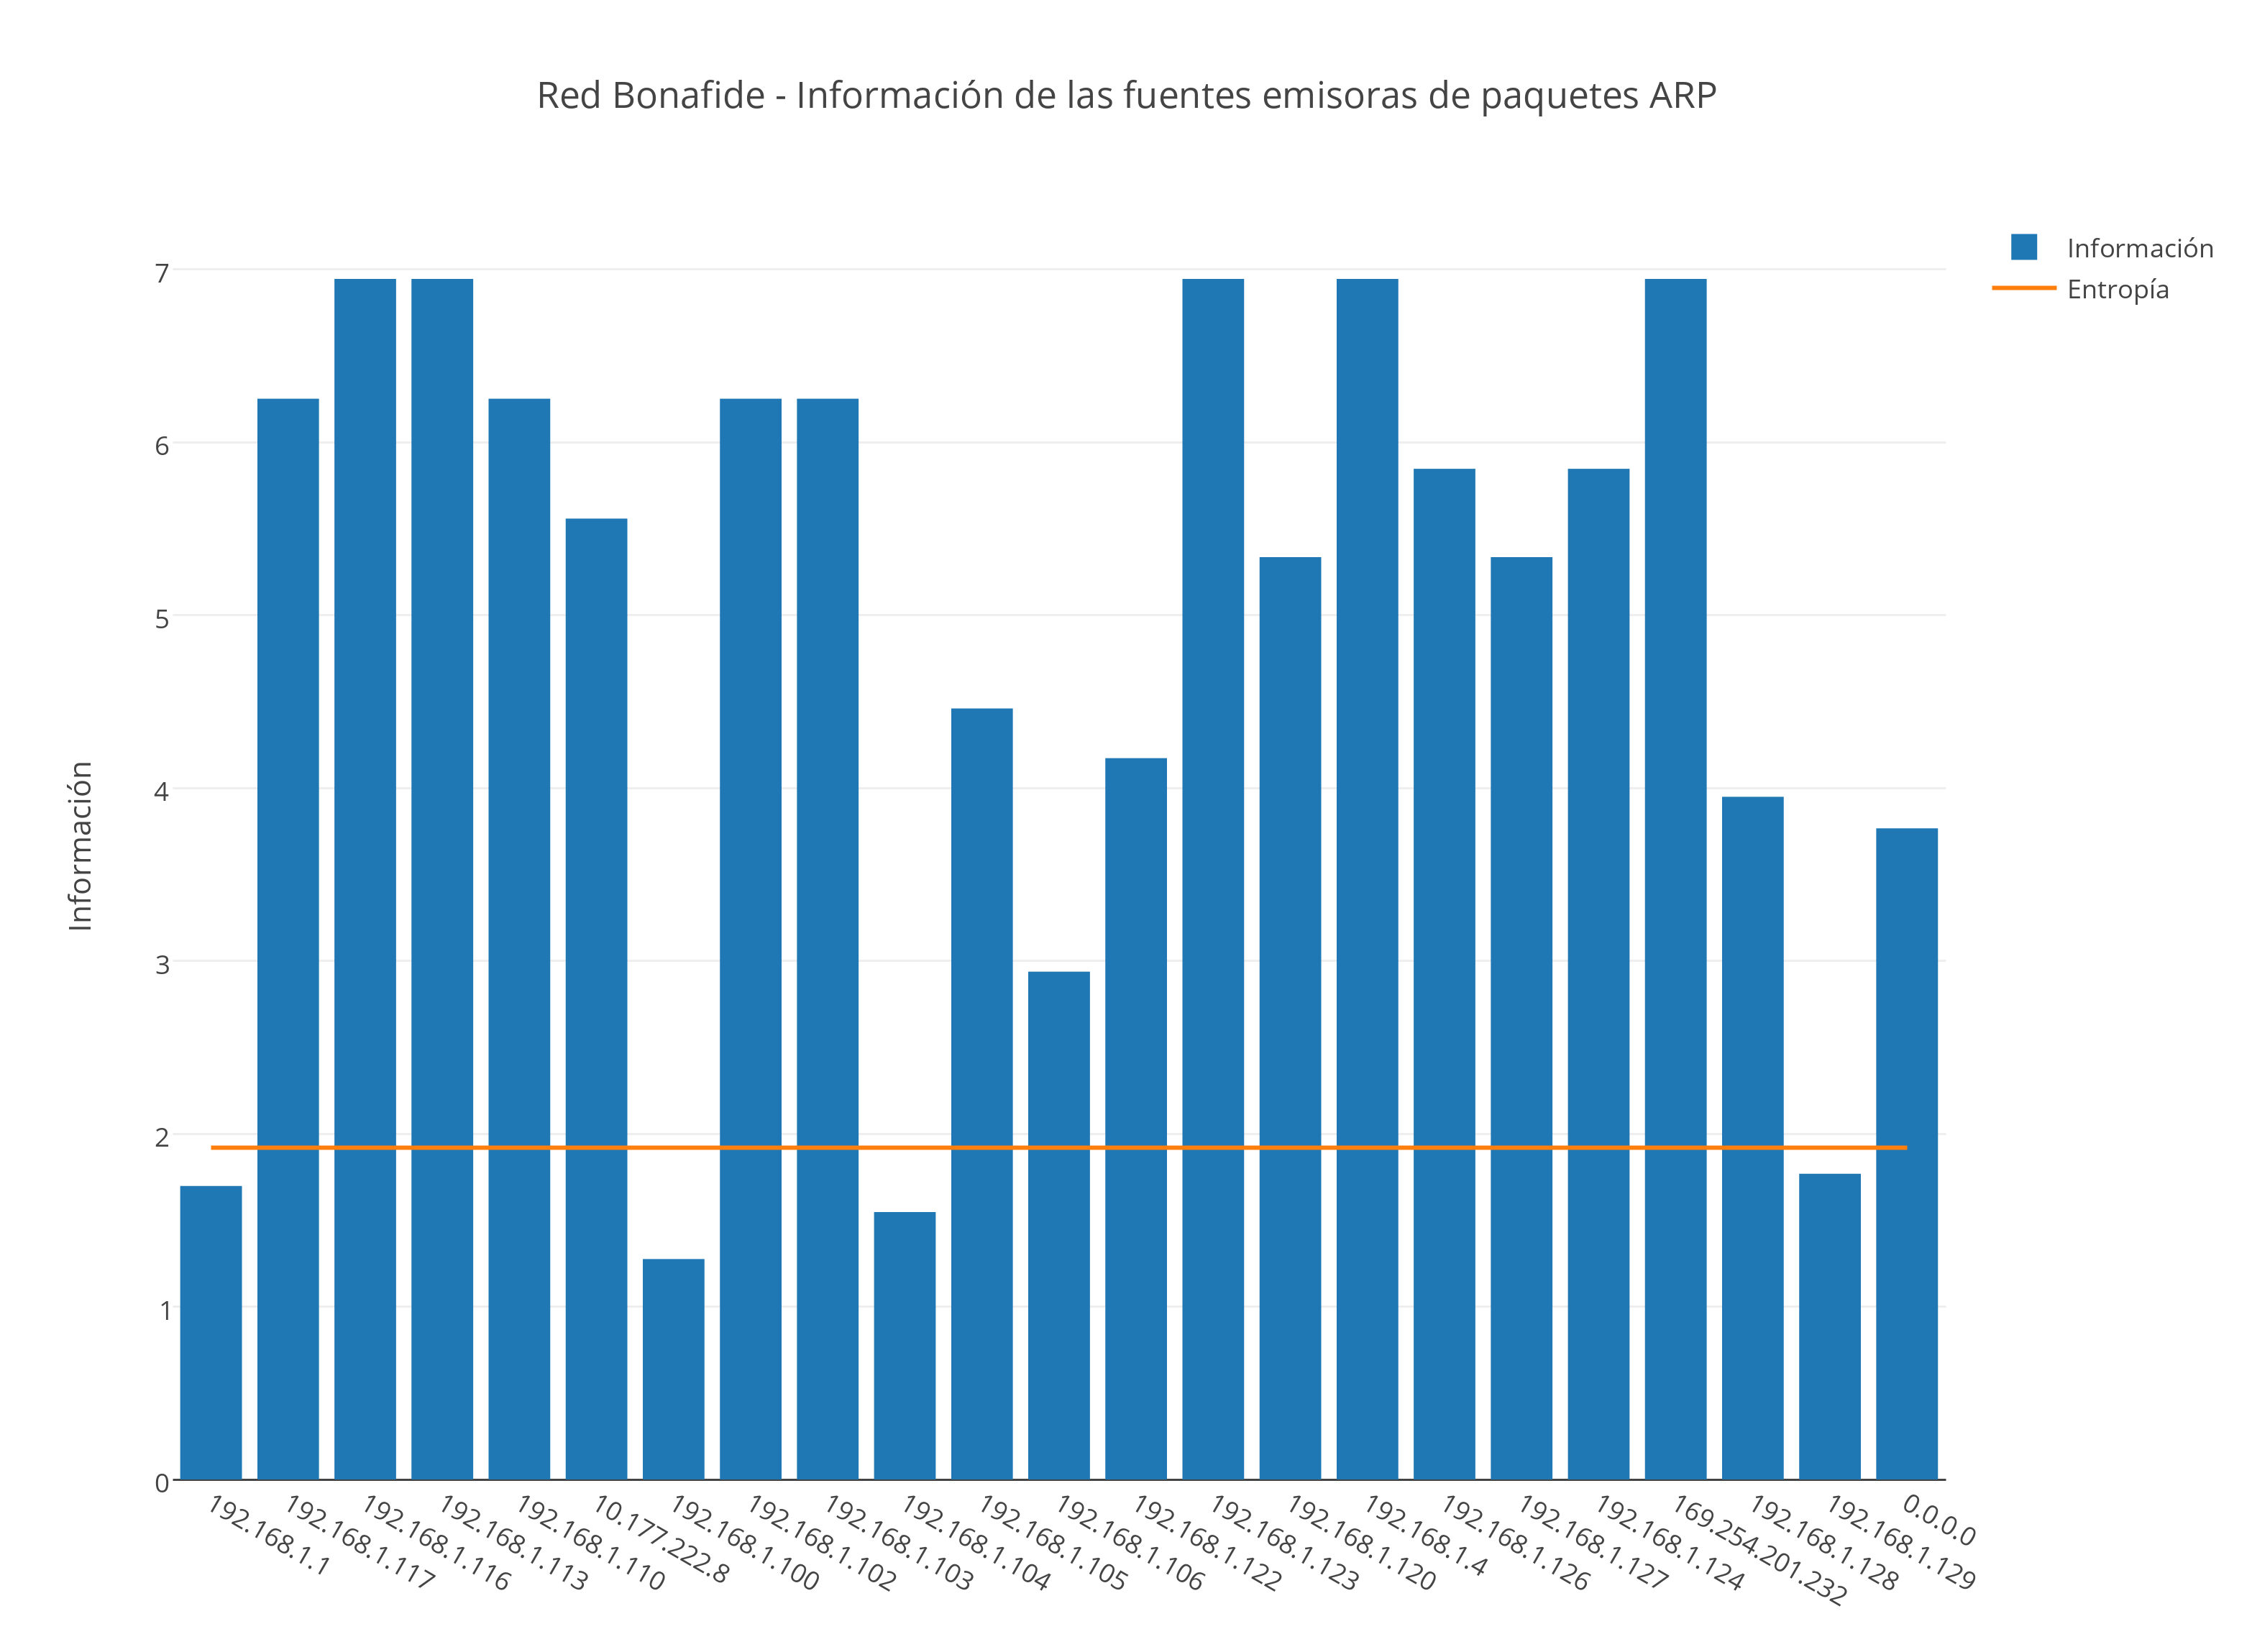
\includegraphics[width=400pt]{img/RedBonafideFuentesEmisorasARP}
    \caption{}
    \label{bonafideEmisoras}
\end{figure}

\begin{figure}[h!]
    \centering                                                       
    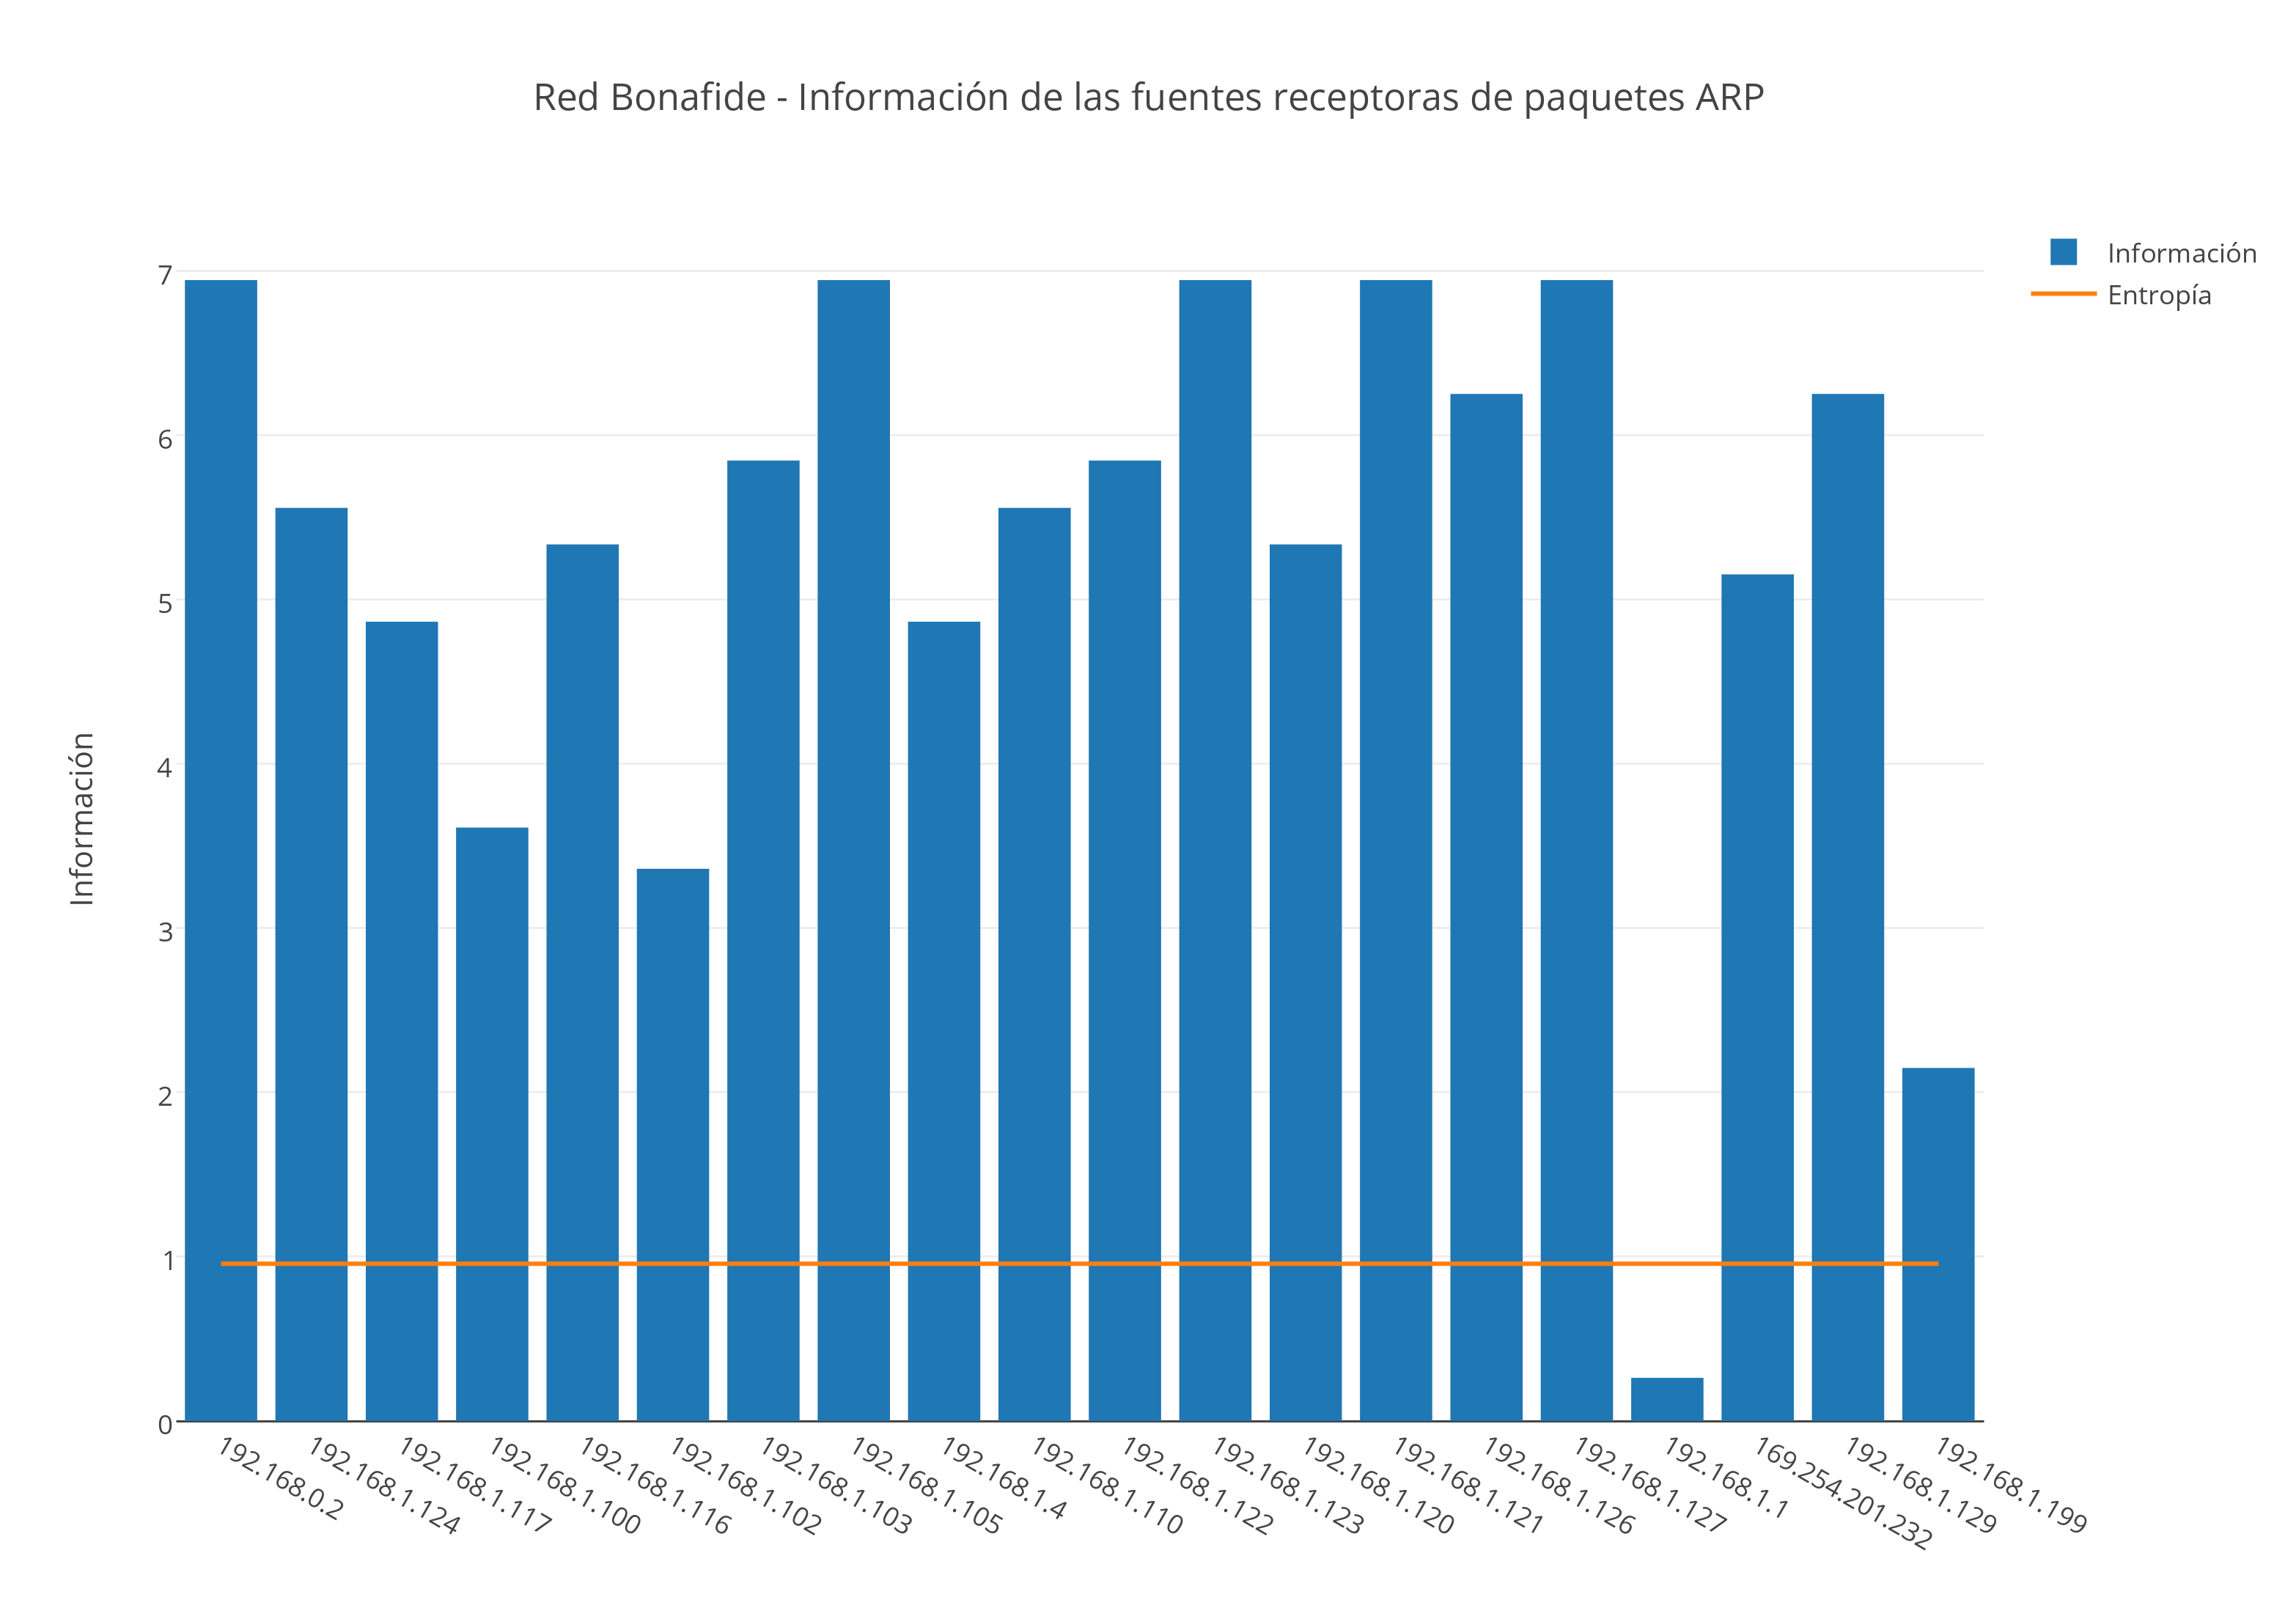
\includegraphics[width=400pt]{img/RedBonafideFuentesReceptorasARP}
    \caption{}
    \label{bonafideReceptoras}
\end{figure}




% \indent Vamos a comenzar mencionando ciertas particularidades que notamos al mirar un poco los datos:
% \begin{itemize}
% 	\item Por los n\'umeros de las direcciones IP, se trata de una red clase A (dentro del rango 0.0.0.0 a 127.255.255.255).
% 	\item A diferencia de lo usual, los que suponemos, son routers, tienen direcciones que terminan distinto a ``.1'' (por ejemplo: ``.254'' o ``.230''). Eso es configurable por el administrador de red, y seg\'un pudimos averiguar, aparte de estilarse tener los \textit{gateway} finalizando en ``.1'', tambi\'en se suele guardar las primeras direcciones para nodos particulares como servidores o impresoras, dejando las \'ultimas direcciones para gateways, como inferimos que sucede en este caso.
% \end{itemize}
% \indent Para no repetir el an\'alisis granular similar al punto anterior, vamos a trabajar con la muestra grande, que se corresponde con todos los paquetes capturados.

% \indent Las entrop\'ias calculadas para ambas fuentes son:\\

% \begin{center}
% 	\begin{tabular}{ | c | c | c |} \hline
% 	   & \textbf{$S_{src}$} & \textbf{$S_{dst}$} \\ \hline
% 	  	\textbf{Entrop\'ia} & 6,29 bits & 5,40 bits \\ \hline
% 	\end{tabular}
% \end{center}

% \indent Como en los an\'alisis anteriores, se realizaron gr\'aficos de barras con la informaci\'on contenida en los s\'imbolos de las fuente con una recta que representa la entrop\'ia de la fuente para contrastar. Recordamos que solamente mostramos en los gr\'aficos los s\'imbolos con menor informaci\'on, es decir aquellos que son suficientes para realizar el an\'alisis pertinente.\\

% \indent Para la fuente \textit{Fuente}, se obtuvo el siguiente gr\'afico:\\

% \begin{center}
% \includegraphics[scale=0.5,clip=true,trim=100 0 0 0]{graphics/facultad_grande_src.png}
% \end{center}

% \indent En contraste con los casos de estudio anteriores, parecer\'ia que aqu\'i una mayor cantidad de nodos cumplen con el criterio que establecimos para ser considerados como nodos distinguidos. El que menos informaci\'on contiene es la IP 10.2.100.254.\\

% \indent Para la fuente destino:\\
% \begin{center}
% \includegraphics[scale=0.5,clip=true,trim=100 0 0 0]{graphics/facultad_grande_dst.png}
% \end{center}
% \indent Se pueden observar claramente cuatro IPs que podr\'iamos considerar distinguidas y una, la 169.254.255.255 con un valor muy similar a la entrop\'ia de la fuente.\\

% \indent Concentr\'andonos en estos candidatos de nodos distinguidos, analizamos el grafo dirigido que representa la captura con el fin de determinar si los resultados se verifican gr\'aficamente como nodos relevantes. Logramos ver que efectivamente hay una relaci\'on, y los nodos que sobresalen en los gr\'aficos. son los que m\'as flechas tienen (desde o hacia ellos, seg\'un corresponda) en los grafos.\\
% \\
% \indent Esta ser\'ia toda la red:\\
% \begin{center}
% \includegraphics[scale=0.5,clip=true,trim=140 0 0 0]{graphics/toda_la_red.png}
% \end{center}
% \newpage
% \indent Por supuesto, este gr\'afico no parece indicarnos nada a esta escala.\\
% \indent Si nos acercamos a algunos de los que catalogamos distinguidos, como el nodo 0.0.0.0 del que salen muchos pedidos y no llega ninguno (en sinton\'ia con el an\'alisis realizado que determinaba que era un nodo distinguido para la fuente origen), y el que suponemos es un router (10.2.100.254) del que salen y llegan muchos pedidos, justificando su aparici\'on como nodo distinguido en ambas fuentes:\\

% \begin{center}
% \includegraphics[scale=0.5,clip=true,trim=140 0 0 0]{graphics/distinguidos.png}

% \includegraphics[scale=0.3,clip=true,trim=140 0 0 0]{graphics/distinguido_todos_ceros.png}

% \includegraphics[scale=0.3,clip=true,trim=140 0 0 0]{graphics/distinguido_router.png}
% \end{center}

% \newpage
% \indent Por \'ultimo, queremos dejar sentada nuestra suposici\'on respecto al subneteo y a las m\'ascaras utilizadas. Seg\'un las caracter\'isticas de las direcciones, nos parece correcto asumir que la m\'ascara aplicada en esta red es una /16, dado que todas las direcciones privadas de la red comienzan en ``10.2''. A su vez, creemos que podemos inferir que el tercer n\'umero en la direcci\'on indica una subred, y las 255 direcciones restantes son los identificadores \'unicos de cada m\'aquina en dicha subred. Esto es respaldado por la forma que tienen las distintas partes del grafo que describe a la red. Estas ser\'ian algunas de las subredes:\\

% \includegraphics[scale=0.5,clip=true,trim=140 0 0 0]{graphics/subnet_1.png}

% \indent Es interesante notar que las IP's 10.2.1.130, 10.2.1.149 y 10.2.1.254 parecen relevantes viendo el gr\'afico siendo receptores de muchos pedidos, lo cual se condice con el hecho de que sean nodos distinguidos para la fuente destino. Adem\'as se observa que muchas de los nodos que distinguimos para la fuente origen aparecen como fuente en paquetes ARP que contiene como direcci\'on destino a las tres IP's mencionadas.\\


% \includegraphics[scale=0.5,clip=true,trim=140 0 0 0]{graphics/subnet_5.png}

% \indent Este \'ultimo gr\'afico es a efectos de mostrar otra subred, aunque sus nodos no son relevantes de acuerdo al an\'alisis que realizamos.\\


\section{Conclusiones}

Al comenzar a resolver los problemas presentados ten\'iamos una idea poco pulida acerca de las redes en general. Conjetur\'abamos ideas respecto a sus estructuras y comportamientos que se vieron refutadas durante el desarrollo y an\'alisis del presente trabajo pr\'actico. Por poner un ejemplo, esper\'abamos encontrar redes cuyo grafo fuese un \'arbol estrella, con el centro como Router y donde no hubiese ciclos ni conexi\'on alguna entre los nodos secundarios. Asimismo, hicieron su aparici\'on direcciones IP que no ten\'iamos presentes.\\
Luego de concretar los experimentos realizados presentamos sus resultados de una forma que consideramos apropiada estudiamos sus resultados, destacando nodos que consideramos distinguidos, investigando el motivo de los resultados imprevistos, obteniendo datos (como la informaci\'on de diversos eventos y la entrop\'ia de una variada cantidad de fuentes) y reuniendo para el an\'alisis integral los datos proporcionados por distintas herramientas que generamos.\\
Luego de todo este proceso, concluimos que:
\begin{itemize}
	\item el c\'alculo de la entrop\'ia resulta imprescindible para conocer la predictibilidad de la fuente que se estudia. 
	\item Es posible deducir con cierta confianza cu\'al es el Router de una red a partir de las interacciones en las que se involucra pasiva o activamente cada host: es, generalmente, el que mayor actividad tiene por su alta intervenci\'on como mediador entre m\'aquinas.
    \item El protocolo ARP es fundamental para la traducci\'on entre direcciones de nivel de red (IP) y direcciones de nivel de enlace (MAC).  
\end{itemize}
